\chapter{Cardiac Electrophysiology}

\section{Cardiac cells}

The cardiac cell membrane is more complicated that that of the squid axon.
Consider the idealised cardiac cell shown in \figref{fig:cardiacmembrane}.  In
addition to the sodium and potassium channels cardiac cells (like other muscle
cells) also have calcium channels. Calcium plays an important role in muscle
contraction and will be covered in more detail in
\secref{sec:excitationcontraction}. For now we will just say that the level of
contraction of a muscle is directly dependent on the amount of calcium in the
cell. The more the calcium the more the contraction.

\pstexfigure{cardiac_electrophysiology/figs/cardiacmembrane.pstex}{}
{Idealised cardiac cell.}{fig:cardiacmembrane}

We will now consider each of the currents and ion pumps in turn. In particular
we will interpret the currents in the same manner as
\citeasnoun{difrancesco:1985}.

%===================================================================
\section{Units}
\label{sec:Units}
%===================================================================
One of the main difficulties encountered when modelling cardiac electrical
activity is that many of the models, both cellular and distributed have
different sets of units. The following standard sets of units have been used
for models presented here \tabref{tab:consist_units}.
\begin{table}[hbtp] \centering
  \begin{tabular}{|c|c|}
    \hline
    \emph{Parameter} & \emph{Units} \\ 
    \hline
    \hline 
     Length & $\mm$ \\
     Area & $\mm^2$ \\
     Volume & $\mm^3$ \\
     Time &  $\ms$ \\
     Voltage & $\mV$ \\
     Current & $\uA$ \\
     Conductivity & $\mS$  \\
     Membrane conductance & $\mS\unitseparator\mm^{-2}$ \\
     Tissue conductivity & $\mS\unitseparator\mm^{-1}$ \\
     Current density & $\uA\unitseparator\mm^{-2}$  \\
     Volume current & $\uA\unitseparator\mm^{-3}$  \\
     Charge & $\nC$  \\
     Capacitance & $\uF$  \\
     Specific capacitance & $\uF\unitseparator\mm^{-2}$  \\
     Concentration & $\nM\unitseparator\mm^{-3} = \mM$  \\ 
     Energy & $\pJ$  \\ 
     Temperature & $\degK$  \\ 
    \hline
  \end{tabular}
  \caption[Consistent units set]{The consistent set of units chosen for all
    models}
  \label{tab:consist_units}
\end{table}


\subsection{Cardiac Ionic Currents}

There are six main ionic currents in the diFrancesco-Noble model of cardiac
electrical activity. These currents are shown graphically in
\figref{fig:diFNcurrents}.
\begin{enumerate}
\item Fast sodium current, $i_{Na}$: Inward, fast, time dependent, $m^{3}h$
  gates.  Activates at $-60$ \mV. Inactivation is very fast and is complete by
  the time the membrane repolarises to $+30$ \mV. Blocked by Tetrodotoxin (TTX)
  from puffer fish.
\item Secondary inward calcium current, $i_{si}$: Inward, slow, time
  dependent, $d$ \& $f$ gates. Activates at $-40$ \mV. This current is very
  small in the Purkinje fibres but is enhanced by nor-adrenaline which enable
  the Purkinje fibres to support pacemaker activity alone. Blocked by
  Nifedipine and Verapamil.
\item Time independent background potassium current, ${i_{K}}_{1}$: Outward,
  time independent. Inward rectifier. At membrane potentials
  between $0$ and $E_{K}$ the current is outward (repolarising), but
  falls drastically at membrane potentials above $0$ \mV. This prevents an
  inefficient loss of \ion{K}{+} ions during the action potential. This
  current is not present in the SA node. The high conductance of this channel
  at -'ve membrane potential is responsible for the resting potential of 
  $-85$ \mV for cardiac cells.
\item Transient outward current, ${i_{t}}_{o}$: time dependent, $r$ gates.
  When activated in sufficient quantities it is characterised by a
  repolarising notch. It involves mainly \ion{K}{+} ions. It is activated by
  intra-cellular calcium.
\item Time dependent potassium current, $i_{K}$ or $i_{x}$: Outward, $x$
  gates. Activates at +'ve membrane potential and deactivates at -'ve
  membrane potential. It behaves as a delayed rectifier and hence repolarises
  membrane. It has slow kinetics which results in a long action potential.
\item Hyperpolarising-activated current, $i_{f}$: Inward, Time
  independent. Activated at -'ve membrane potentials and deactivated at +'ve
  membrane potentials. Reversal potential at $-30$ \mV hence the current is
  inward at the resting potential.
\end{enumerate}

\pstexfigure{cardiac_electrophysiology/figs/diFNcurrents.pstex}{}
{diFrancesco-Noble currents making up the cardiac action potential. Note all
  conductances are \tento{-4}\units{S/cm^2}.}{fig:diFNcurrents}

\section{Ion Pumps and Exchanges}

There are two main ion pumps and one ion exchanger in cardiac cells.
\begin{enumerate}
\item Sodium-Potassium pump , $i_{NaK}$: Pumps $3$ \ion{Na}{+} ions out of the
  cell and brings in $2$ \ion{K}{+} ions. It is \emph{electrogenic}, that is
  there is a net transfer of charge, and ATP (Adenosine Tri-Phosphate)
  dependent. It is blocked by the cardiac glycosides (e.g. digitalis, ouabain)
  and vanadium. It is this pump that maintains the resting potential. The
  density of the sodium pump is about $400$ per \units{\mu m^2} of sarcolemma
  ($\sim$ $\tento{6}$ in a cell), compared with $16$ for the sodium channel
  and $0.1$ for the calcium channel.
\item Calcium pump: Mainly in the sarcoplasmic reticulum. ATP dependent. It
  is much slower than the sodium-calcium exchange.
\item Sodium-Calcium exchange, $i_{NaCa}$: Transfers $3$ \ion{Na}{+} ions into
  of the cell and removes $1$ \ion{Ca}{2+} from the cell. Works on a
  concentration gradient and is hence enhanced by increased
  $\conc{\ion{Ca}{2+}}{i}$ or $\conc{\ion{Na}{+}}{o}$. It is not ATP dependent
  and is faster and about $30$ times more effective that the calcium pump. It is
  voltage dependent and has a reversal potential of $+20$ \mV.
\end{enumerate}

\section{diFrancesco-Noble Model}

The diFrancesco-Nobel model of the cardiac action potential is summarised
by \figref{fig:diFNactionpot}.

\pstexfigure{cardiac_electrophysiology/figs/diFNactionpot.pstex}{}{diFrancesco-Noble action potential
  currents for cardiac cells.}{fig:diFNactionpot}

\section{Changes in the action potential}

Consider the following changes in the action potential
\begin{enumerate}
\item Increase in extra-cellular calcium. Intra-cellular calcium is increased
  as more calcium enters the cell from the extra-cellular space. Force is
  hence increased due to the increased intra-cellular calcium. The action
  potential is prolonged because the intra-cellular calcium is increased. This
  results in an increase in the sodium calcium exchange current prolonging the
  plateau of the action potential.
\item Decrease in extra-cellular sodium. Force increases as the sodium-calcium
  exchange is decreased resulting in increased intra-cellular calcium. The
  action potential is shortened.
\item Addition of Nifedipine (a calcium channel blocker). Force is decreased
  as calcium cannot enter the cell to interact with the contractile
  proteins. The action potential is shortened due to the decrease in the
  secondary inward calcium current and decrease in the sodium-calcium
  exchange.
\item Addition of Digitalis (which inhibits the 3\ion{Na}{+}/2\ion{K}{+}
  pump). Force is increased as intra-cellular sodium is increased which results
  in a decreased calcium efflux through the sodium-calcium exchange.
\item Addition of caffeine (releases calcium from the mitochondria). Increases
  the intra-cellular calcium and hence increases force. The action potential
  plateau is extended as the increased intra-cellular calcium is removed via
  the sodium-calcium exchange. This is shown in \figref{fig:caffeineeffect}.
\end{enumerate}

\pstexfigure{cardiac_electrophysiology/figs/caffeineeffect.pstex}{}{Effect of
  caffeine on the cardiac action potential.}{fig:caffeineeffect}

\section{Other membrane models}
\label{sec:biophysical_models_of_cardiac_cells}
%===================================================================
\subsection{The Beeler-Reuter model}
\label{sec:The_Beeler-Reuter_model}
%===================================================================
There are many other models of cellular electrophysiology, and we present some
of them here.  The Beeler-Reuter is the simplist physiologically-based model.
The model developed by Beeler and Reuter \cite{beeler:1977} is specifically a model of
mammalian ventricular myocardial cells. The standard model is based around
ionic current densities across $1 \cm^2$ so it was necessary to convert the
units of the ionic currents and also the calcium ion concentration. Four
currents are present in the model, they are an fast inward sodium current,
$I_{Na}$, an outward time independent potassium current, $I_{K1}$, a time
dependent outward current based mainly on potassium ions, $I_{x1}$ and a slow
inward current $I_{s}$ which is 
mainly due to calcium ion transfer. The ionic current model may be written as
\begin{equation}
  I_{ion} = I_{Na} + I_{K1} + I_{x1} + I_{s}
  \label{eqn:BeelerReuter_ionic_current_model}
\end{equation}
\incgrfigure{width=75mm}{cardiac_electrophysiology/epsfiles/BR_Vm.eps}{Beeler-Reuter
  action potential}{Action potential trace from the Beeler-Reuter
  ionic current model.}{fig:BR_ap}
All currents in the model have been converted into units of
$\uA\unitseparator\mm^{-2}$ to maintain consistency with the diffusive
processes. $I_{Na}$ was responsible for the fast upstroke of the action
potential and $I_s$ was responsible for the duration of the plateau phase. The
two potassium currents, $I_{K1}$ and $I_{x1}$ were responsible for the
repolarization of the cell. The action potential generated by the
Beeler-Reuter model is shown in \figref{fig:BR_ap}.

\subsubsection{Fast inward sodium current}
\enlargethispage{-\baselineskip}
\enlargethispage{-\baselineskip}
\enlargethispage{-\baselineskip}
\enlargethispage{-\baselineskip}
\enlargethispage{-\baselineskip}
The fast inward sodium current is controlled by three gating variables which
follow the standard Hodgkin-Huxley formulation. The $m$ gate is the activation
gate and the $h$ gate is the inactivation gate. In addition to this there is a
slow inactivation gate $j$. The magnitude of this current was defined to be
\begin{equation}
  I_{Na}=\pbrac{\overline{g_{Na}}\cdot m^3\cdot h\cdot
    j+\overline{g_{NaC}}}\cdot \pbrac{V_m-E_{Na}}
\end{equation}
where $E_{Na}$ is the sodium reversal potential which was set at $50\mV$ and
$\overline{g_{Na}}$ is the fully activated sodium conductance at $4\times 10^{-2}
\mS\unitseparator\mm^{-2}$. $\overline{g_{NaC}}$ is the steady state sodium conductance
which was set to be $3\times 10^{-5} \mS\unitseparator\mm^{-2}$. The time
dependence of the gating variables was defined as
\begin{align}
  \label{eqn:br_mt}
  \dby{m}{t}=&\alpha_m\cdot \pbrac{1-m}-\beta_m\cdot  m \\
  \label{eqn:br_ht}
  \dby{h}{t}=&\alpha_h\cdot \pbrac{1-h}-\beta_h\cdot  h \\
  \label{eqn:br_jt}
  \dby{j}{t}=&\alpha_j\cdot \pbrac{1-j}-\beta_j\cdot  j
\end{align}
where the rate constants were given by
\begin{align}
  \alpha_m =& \dfrac{-\pbrac{V_m+47}}{\exp\pbrac{-0.1\pbrac{V_m+47}}-1} \\
  \beta_m =& 40\exp\pbrac{-0.056\pbrac{V_m+72}} \\
  \alpha_h =& 0.126\exp\pbrac{-0.25\pbrac{V_m+77}} \\
  \beta_h =& \dfrac{1.7}{\exp\pbrac{-0.082\pbrac{V_m+22.5}}+1} \\
  \alpha_j =& 0.055\sqbrac{\dfrac{\exp\pbrac{-0.25\pbrac{V_m+78}}}{\exp\pbrac{-0.2\pbrac{V_m+78}}+1}} \\
  \beta_j =&  \dfrac{0.3}{\exp\pbrac{-0.1\pbrac{V_m+32}}+1}
\end{align}
The fast inward sodium current and the gating variables are shown in
\figref{fig:BR_NA_traces}.

\begin{figure}[hbtp]
  \centering
  \begin{subfigure}[b]{0.45\linewidth}
    \centering
    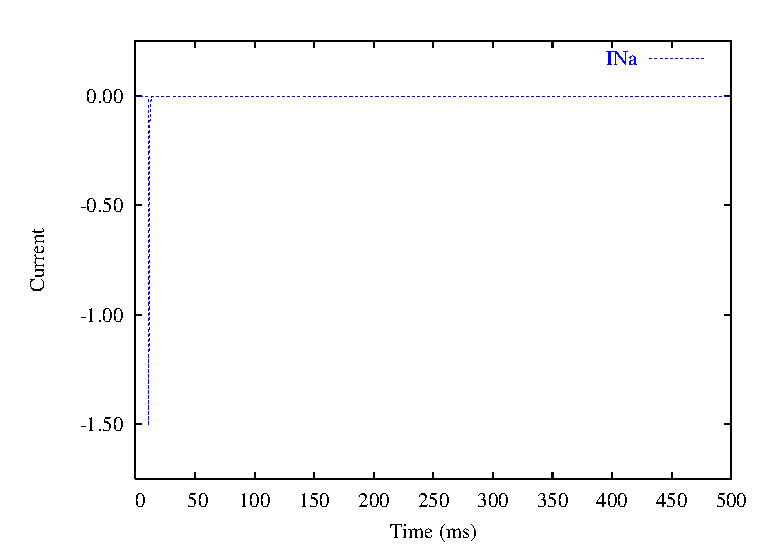
\includegraphics[width=\textwidth]{cardiac_electrophysiology/epsfiles/BR_INa.eps}
    \caption{}
  \end{subfigure}
  \hfill
  \begin{subfigure}[b]{0.45\linewidth}
    \centering
    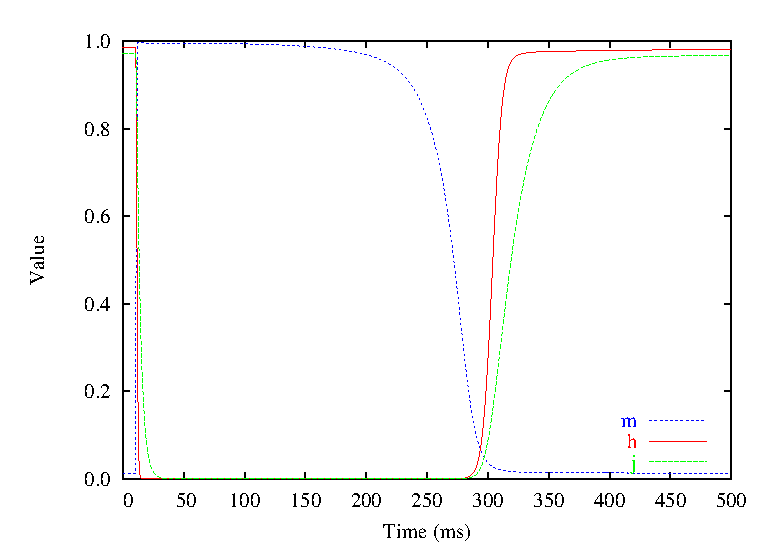
\includegraphics[width=\linewidth]{cardiac_electrophysiology/epsfiles/BR_mhj.eps} \\
    \caption{}
  \end{subfigure}
  \caption[Fast inward sodium current from the Beeler-Reuter model]{Figure(a) shows the
    fast inward sodium current over time and Figure(b) shows the $m$, $h$ and
    $j$ gate variables over time from the Beeler-Reuter model.}
  \label{fig:BR_NA_traces}
\end{figure}
%
\subsubsection{Time independent outward potassium current}
The magnitude of the time independent outward potassium current, $I_{K1}$ was
given by 
\begin{equation}
  I_{K1}=0.0035\sqbrac{\dfrac{4\pbrac{\exp\pbrac{0.04\pbrac{V_m+85}}-1}} 
    {\exp\pbrac{0.08\pbrac{V_m+53}}+\exp\pbrac{0.04\pbrac{Vm+53}}} 
    +\dfrac{0.2\pbrac{V_m+23}} {1-\exp\pbrac{-0.04\pbrac{V_m+23}}}} 
\end{equation}
and the temporal trace of the current is shown in \figref{fig:BR_ik1}.
\begin{figure}[hbtp] 
  \centering
  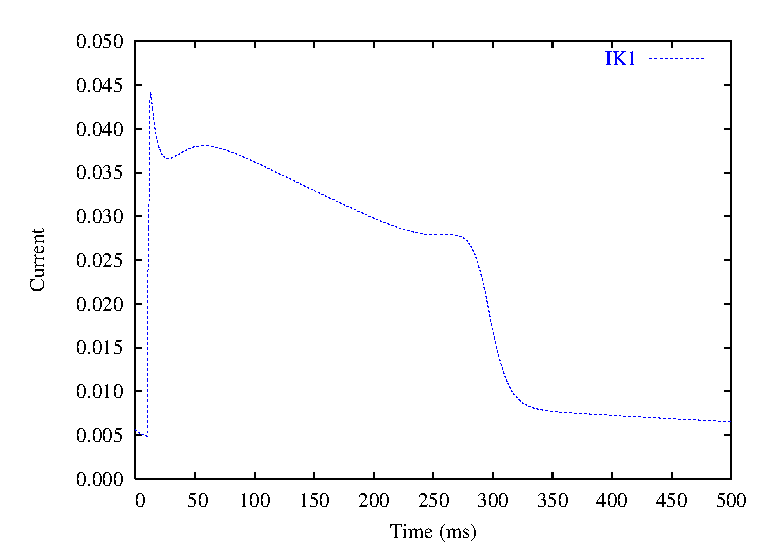
\includegraphics[width=75mm]{cardiac_electrophysiology/epsfiles/BR_IK1.eps}
  \caption[Beeler-Reuter time independent potassium current]{The time
    independent outward potassium current from the Beeler-Reuter model.}
  \label{fig:BR_ik1}
\end{figure}
%
\subsubsection{Time dependent outward potassium current}
The time dependent outward potassium current was controlled by a single
Hodgin-Huxley type gating variable, $x_1$.
\begin{equation}
  I_{x1}=8\times 10^{-3}\cdot x_1\cdot \sqbrac{\dfrac{\exp\pbrac{0.04\pbrac{V_m+77}}-1}
    {\exp\pbrac{0.04\pbrac{V_m+35}}}}
\end{equation}
where the time dependence of $x_1$ was defined to be 
\begin{equation}
  \dby{x_1}{t}=\alpha_{x1}\cdot\pbrac{1-x_1}-\beta_{x1}\cdot x_1
\end{equation}
The rate constants were calculated from
\begin{align}
  \alpha_{x1} =& 5\times 10^{-4}\sqbrac{\dfrac{\exp\pbrac{0.083\pbrac{V_m+50}}}
    {\exp\pbrac{0.057\pbrac{V_m+50}+1}}} \\
  \beta_{x1} =& 1.3\times 10^{-3}\sqbrac{\dfrac{\exp\pbrac{-0.06\pbrac{V_m+20}}}
    {\exp\pbrac{-0.04\pbrac{V_m+20}+1}}}
\end{align}
The size of the current and state of the gating variable over time are shown
in \figref{fig:BR_Ix1_traces}.
\begin{figure}[hbtp] 
  \centering
  \begin{subfigure}[b]{0.45\linewidth}
    \centering
    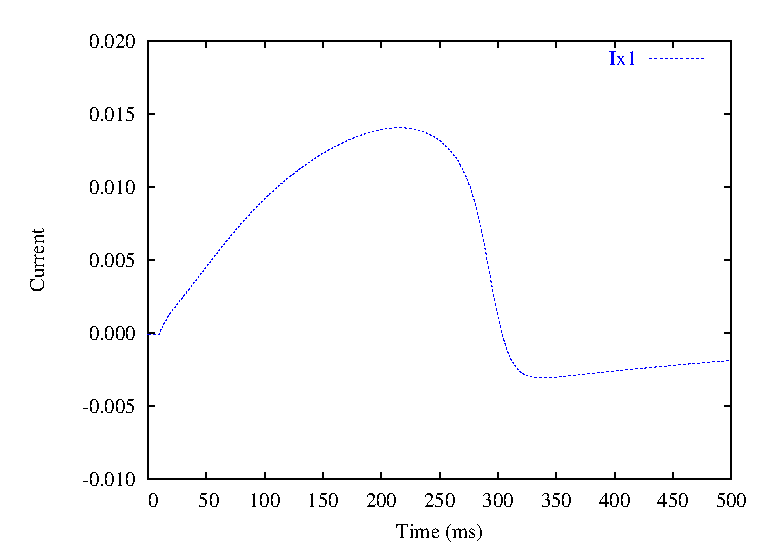
\includegraphics[width=\textwidth]{cardiac_electrophysiology/epsfiles/BR_Ix1.eps}
    \caption{}
  \end{subfigure}
  \hfill
  \begin{subfigure}[b]{0.45\linewidth}
    \centering
    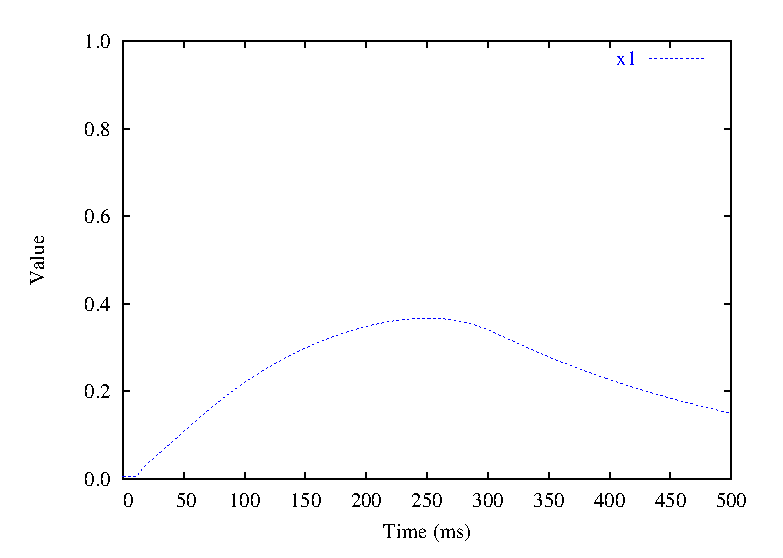
\includegraphics[width=\textwidth]{cardiac_electrophysiology/epsfiles/BR_x1.eps}
    \caption{}
  \end{subfigure}
  \caption[Beeler-Reuter time dependent potassium current]{Figure(a) shows the
    time dependent outward potassium current over time and Figure(b) shows the
    $x_1$ gate variable over time from the Beeler-Reuter model.}
  \label{fig:BR_Ix1_traces}
\end{figure}
%
\subsubsection{Slow inward current}
The slow inward current was based mainly around the uptake of calcium ions
into the cell. The current features an activation gate $d$ and an inactivation
gate $f$. The ionic current was represented by
\begin{equation}
  I_s=\overline{g_s}\cdot d\cdot f\cdot \pbrac{V_m-E_s}
\end{equation}
where $\overline{g_s}$ is the fully activated channel conductance which was
set to be $9\times 10^{-4}\mS\unitseparator\mm^{-2}$. The reversal potential
for the current was dependent on the concentration of calcium ions present in
the cell.
\begin{equation}
  E_s=-82.3-13.0287\fnof{ln}{0.001\conc{Ca^{2+}}{i}}
\end{equation}
The time dependence of the intracellular calcium concentration was governed by
\begin{equation}
  \dby{\conc{Ca^{2+}}{i}}{t}=-0.01 I_s + 0.07\pbrac{1\times 10^{-4} - \conc{Ca^{2+}}{i}}
\end{equation}
and the concentration is shown in \figref{fig:BR_cai}.
\begin{figure}[hbtp] 
  \centering
  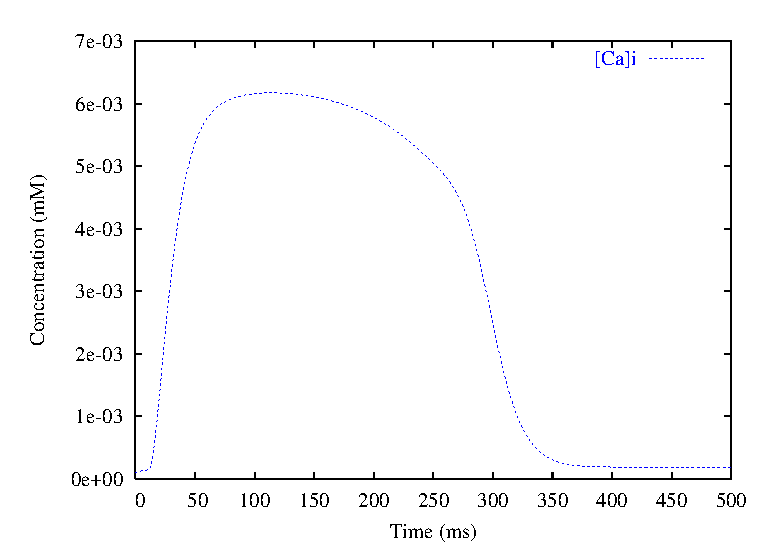
\includegraphics[width=75mm]{cardiac_electrophysiology/epsfiles/BR_Cai.eps}
  \caption[Beeler-Reuter intracellular calcium concentration]{The
    intracellular calcium ion concentration from the Beeler-Reuter model.}
  \label{fig:BR_cai}
\end{figure}
The two gating variables were calculated using
\begin{align}
  \label{eqn:br_dt}
  \dby{d}{t}=&\alpha_{d}\cdot\pbrac{1-d}-\beta_{d}\cdot d \\
  \label{eqn:br_ft}
  \dby{f}{t}=&\alpha_{f}\cdot\pbrac{1-f}-\beta_{f}\cdot f
\end{align}
The values of the rate constants were found from
\begin{align}
  \alpha_{d} =& 0.095\sqbrac{\dfrac{\exp\pbrac{-0.01\pbrac{V_m-5}}}
    {\exp\pbrac{-0.072\pbrac{V_m-5}}+1}} \\
  \beta_{d} =& 0.07\sqbrac{\dfrac{\exp\pbrac{-0.017\pbrac{V_m+44}}}
    {\exp\pbrac{0.05\pbrac{V_m+44}}+1}} \\
  \alpha_{f} =& 0.012\sqbrac{\dfrac{\exp\pbrac{-0.008\pbrac{V_m+28}}}
    {\exp\pbrac{0.15\pbrac{V_m+28}}+1}} \\
  \beta_{f} =& 0.0065\sqbrac{\dfrac{\exp\pbrac{-0.02\pbrac{V_m+30}}}
    {\exp\pbrac{-0.2\pbrac{V_m+30}}+1}}
\end{align}
The magnitude of the current and the state of the gating variables over time
is shown in \figref{fig:BR_Is_traces}.
\begin{figure}[hbtp] 
  \centering
  \begin{subfigure}[b]{0.45\linewidth}
    \centering
    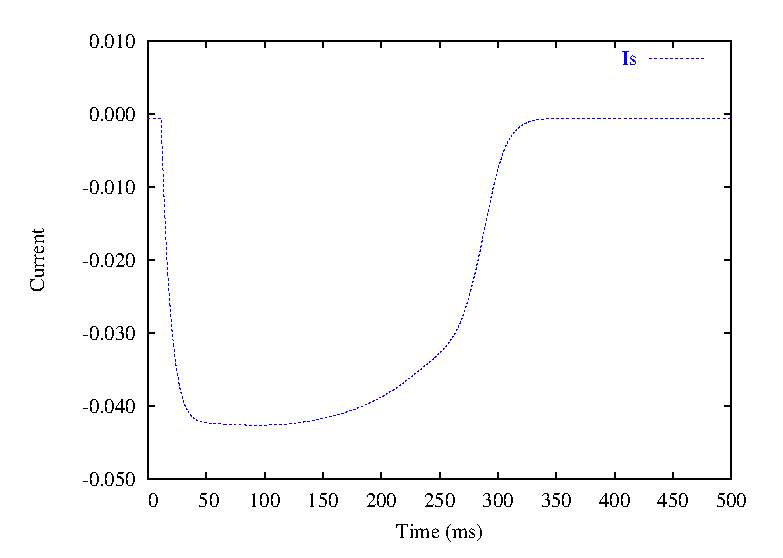
\includegraphics[width=\textwidth]{cardiac_electrophysiology/epsfiles/BR_Is.eps}
    \caption{}
  \end{subfigure}
  \hfill
  \begin{subfigure}[b]{0.45\linewidth}
    \centering
    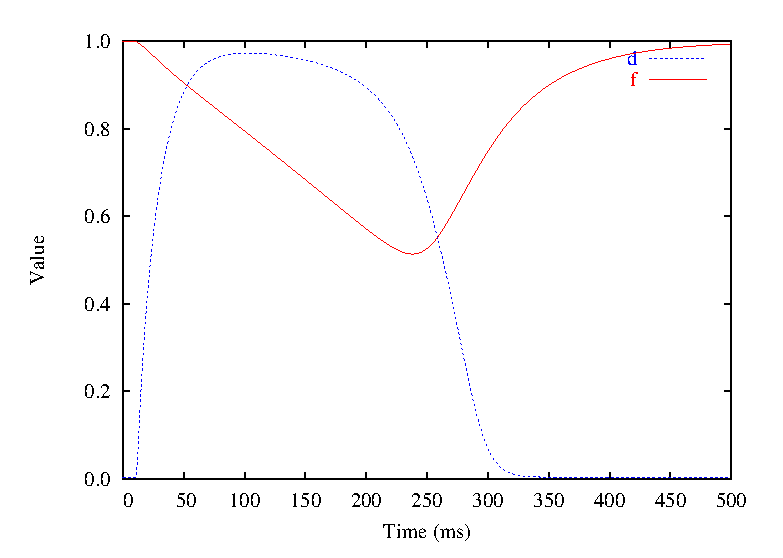
\includegraphics[width=\textwidth]{cardiac_electrophysiology/epsfiles/BR_df.eps}
    \caption{}
  \end{subfigure}
  \caption[Beeler-Reuter slow inward current]{Figure(a) shows the
    slow inward current over time and Figure(b) shows the
    $d$ and $f$ gate variables over time from the Beeler-Reuter model.}
  \label{fig:BR_Is_traces}
\end{figure}
%
The initial values of the gating variables were calculated from the initial
value of the transmembrane potential. The initial value for a gate $i$ was
given by
\begin{equation}
  i=\dfrac{\alpha_i}{\alpha_i+\beta_i}
\end{equation}
The values of the other parameters used in the Beeler-Reuter model whose
values have not yet been specified are given in \tabref{tab:BR_Model_Params}.
\begin{table}[hbtp] \centering
  \begin{tabular}{|c|c|c|}
    \hline
    \emph{Parameter} & \emph{Value} & \emph{Units}  \\ 
    \hline
    \hline 
    $V_m$  & $-84.0$ & $\mV$\\
    $\conc{Ca^{2+}}{i}$  & $1\times 10^{-4}$ & $\nM\unitseparator\mm^{-3}$\\
    $C_m$  & $0.01$ & $\uF\unitseparator\mm^{-2}$\\
    $A_m$ & $200$ & $\mm^{-1}$ \\
    \hline
  \end{tabular}
  \caption[Parameter values used in the Beeler-Reuter model]{Parameter values
    used in the Beeler-Reuter model}
  \label{tab:BR_Model_Params}
\end{table}
%
%===================================================================
\subsection{The defibrillation Beeler-Reuter model}
\label{sec:The_defibrillation_Beeler-Reuter_model}
%===================================================================
The original Beeler-Reuter model was modified by Drouhard and Roberge
to improve the fast sodium current kinetics. This model was then further
modified by \citeasnoun{skouibine:1999} to handle voltages outside the range of normal
physiological activity for use with defibrillation studies. The action
potential for the defibrillation Beeler-Reuter model is shown in
\figref{fig:BRDR_ap}.
\begin{figure}[hbtp] 
  \centering
  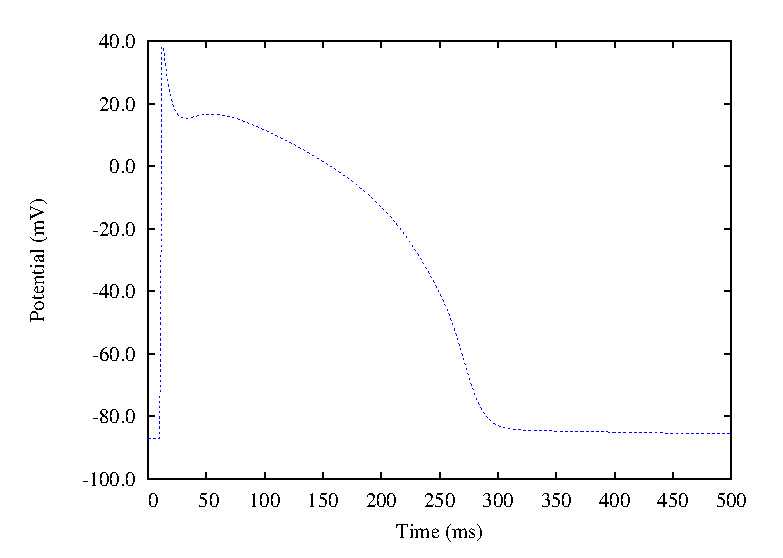
\includegraphics[width=75mm]{cardiac_electrophysiology/epsfiles/BRDR_Vm.eps}
  \caption[Defibrillation Beeler-Reuter action potential]{Action potential
    trace from the defibrillation Beeler-Reuter ionic current model.}
  \label{fig:BRDR_ap}
\end{figure}
%
\subsubsection{Fast inward sodium current}
The steady state sodium conductance, $\overline{g_{NaC}}$ was
removed along with the slow inactivation gating variable $j$ leaving the
following equation for the fast inward sodium current. 
\begin{equation}
  I_{Na}=\overline{g_{Na}}\cdot m^3\cdot h\cdot \pbrac{V_m-E_{Na}}
\end{equation}
where $E_{Na}$ was set to $40\mV$ which is smaller than the standard
Beeler-Reuter model and $\overline{g_{Na}}$ was set to $0.15\mS\unitseparator\mm^{-2}$,
nearly four times larger than in the original model. The gating variables were
altered to cope with the large potentials encountered during defibrillation.
\begin{gather}
  \label{eqn:brdr_ina_coeffs}
  \begin{aligned}
    \alpha_m &=
    \begin{cases}
      0.9\sqbrac{\dfrac{V_m+42.65}{1-\exp\pbrac{\pbrac{-0.22V_m-9.3830}}}}
        & \text{if $V_m \le 100\mV$} \\
      890.9437890\sqbrac{\dfrac{\exp\pbrac{\pbrac{0.0486479V_m-4.8647916}}}
        {1+5.93962526\exp\pbrac{\pbrac{0.0486479V_m-4.8647916}}}}
        & \text{if $V_m > 100\mV$} 
    \end{cases} \\
    \beta_m &=
    \begin{cases}
      1.437\exp\pbrac{\pbrac{-0.085V_m -3.37875}}
        & \text{if $V_m > -85\mV$} \\
      \dfrac{100}{1+\exp\pbrac{\pbrac{0.2597504V_m+22.0787804}}}
        & \text{if $V_m \le -85\mV$} 
    \end{cases} \\
    \alpha_h &=
    \begin{cases}
      0.1\exp\pbrac{\pbrac{-0.193V_m-15.37245}}
        & \text{if $V_m > -90\mV$} \\
      -12.0662845-0.1422598V_m
        & \text{if $V_m \le -90\mV$} 
    \end{cases} \\
    \beta_h &=
    \begin{cases}
      \dfrac{1.7}{1+\exp\pbrac{\pbrac{-0.095V_m-1.9475}}} 
        & \text{for all $V_m$}
    \end{cases}
  \end{aligned}
\end{gather}
The fast inward sodium current and the gating variables are shown in
\figref{fig:BRDR_NA_traces}.
\begin{figure}[hbtp] 
  \centering
  \begin{subfigure}[b]{0.45\linewidth}
    \centering
    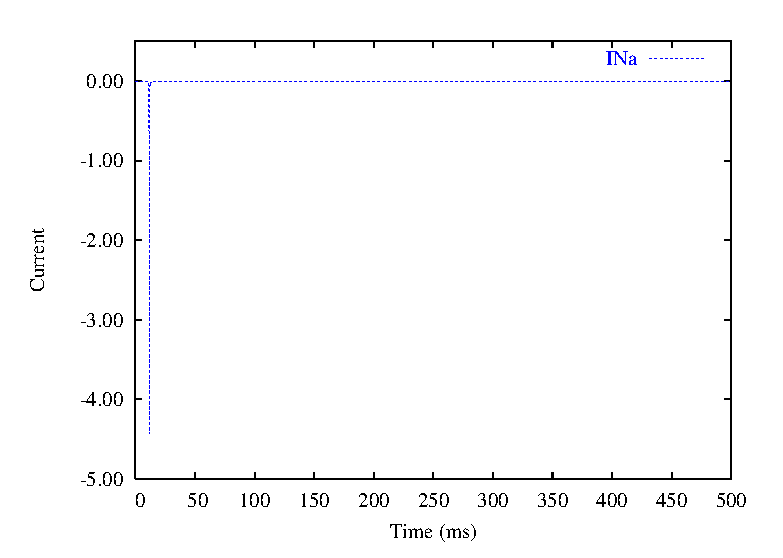
\includegraphics[width=\textwidth]{cardiac_electrophysiology/epsfiles/BRDR_INa.eps}
    \caption{}
  \end{subfigure}
  \hfill
  \begin{subfigure}[b]{0.45\linewidth}
    \centering
    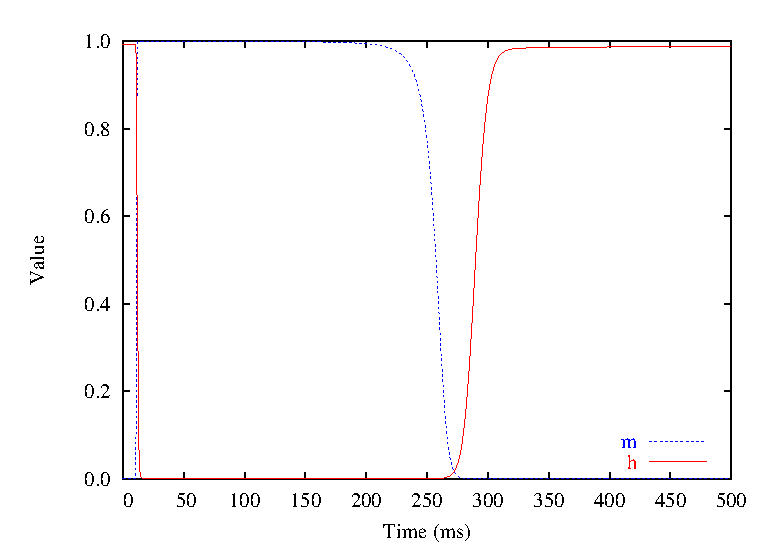
\includegraphics[width=\textwidth]{cardiac_electrophysiology/epsfiles/BRDR_mh.eps}
    \caption{}
  \end{subfigure}
  \caption[Fast inward sodium current from the defibrillation Beeler-Reuter
  model]{Figure(a) shows the 
    fast inward sodium current over time and Figure(b) shows the $m$, and $h$
    gating variables over time from the defibrillation Beeler-Reuter model.}
  \label{fig:BRDR_NA_traces}
\end{figure}
%
\subsubsection{Time independent outward potassium current}
The formula for time independent outward potassium current was unchanged. The
time course of the current is shown in \figref{fig:BRDR_ik1}
\begin{figure}[hbtp] 
  \centering
  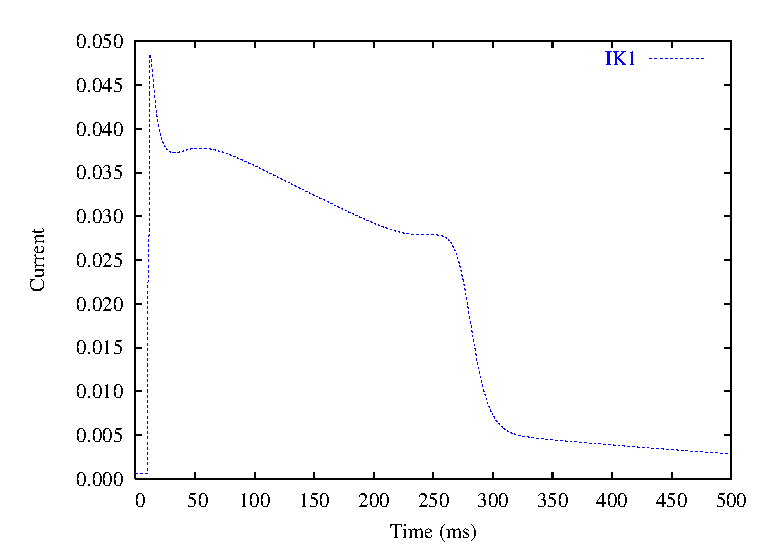
\includegraphics[width=75mm]{cardiac_electrophysiology/epsfiles/BRDR_IK1.eps}
  \caption[Defibrillation Beeler-Reuter time independent potassium current]{The time
    independent outward potassium current from the defibrillation Beeler-Reuter model.}
  \label{fig:BRDR_ik1}
\end{figure}
%
\subsubsection{Time dependent outward potassium current}
While the governing equations for the time dependent outward potassium current
were unchanged, the gating variables were modified to become
\begin{gather}
  \label{eqn:brdr_ix1_coeffs}
  \begin{aligned}
    \alpha_{x1} &=
    \begin{cases}
      0.0005\sqbrac{\dfrac{\exp\pbrac{\pbrac{0.083V_m+4.150}}}
        {\exp\pbrac{\pbrac{0.057V_m+2.850}}+1}}
        & \text{if $V_m \le 400\mV$} \\
      151.7994692\sqbrac{\dfrac{\exp\pbrac{\pbrac{0.0654679V_m-26.1871448}}}
        {1+1.5179947\exp\pbrac{\pbrac{0.0654679V_m-26.1871448}}}}
        & \text{if $V_m > 400\mV$} 
    \end{cases} \\
    \beta_{x1} &=
    \begin{cases}
      0.0013\sqbrac{\dfrac{\exp\pbrac{\pbrac{-0.06V_m-1.20}}}
      {\exp\pbrac{\pbrac{-0.04V_m-0.80}}+1}}
      & \text{for all $V_m$}
    \end{cases}
  \end{aligned}
\end{gather}
The size of the current and state of the gating variable over time are shown
in \figref{fig:BRDR_Ix1_traces}.
\begin{figure}[hbtp] 
  \centering
  \begin{subfigure}[b]{0.45\linewidth}
    \centering
    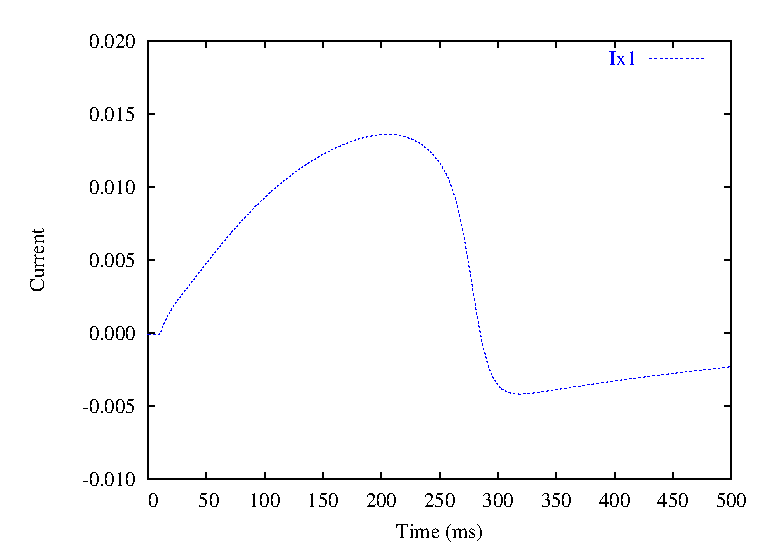
\includegraphics[width=\textwidth]{cardiac_electrophysiology/epsfiles/BRDR_Ix1.eps}
    \caption{}
  \end{subfigure}
  \hfill
  \begin{subfigure}[b]{0.45\linewidth}
    \centering
    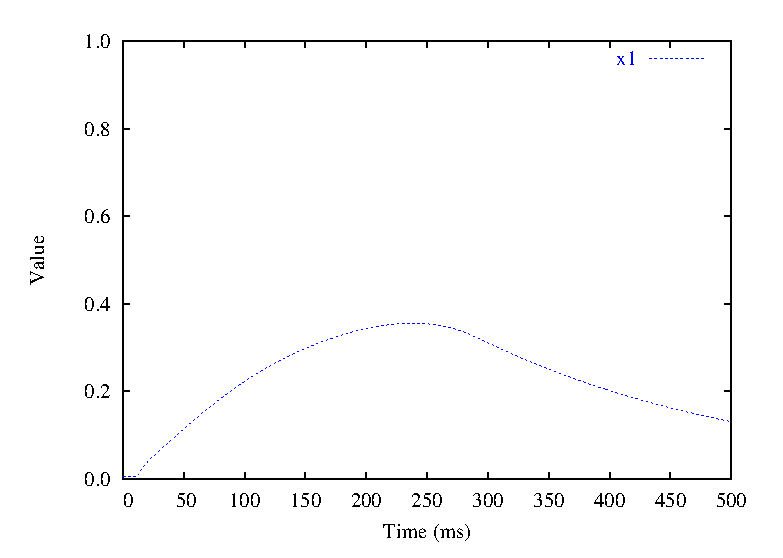
\includegraphics[width=\textwidth]{cardiac_electrophysiology/epsfiles/BRDR_x1.eps}
    \caption{}
  \end{subfigure}
  \caption[Defibrillation Beeler-Reuter time dependent potassium current]{Figure(a) shows the
    time dependent outward potassium current over time and Figure(b) shows the
    $x_1$ gate variable over time from the defibrillation Beeler-Reuter model.}
  \label{fig:BRDR_Ix1_traces}
\end{figure}
%
\subsubsection{Slow inward current}
There was a change made to the intracellular calcium ion tracking in order to
limit the movement of calcium ions at large potentials.
\begin{gather}
  \label{eqn:two_cases_of_caiBRDR}
  \begin{aligned}
    \dby{\conc{Ca^{2+}}{i}}{t} &=
    \begin{cases}
      -0.01 I_s + 0.07\pbrac{1\times 10^{-4} - \conc{Ca^{2+}}{i}}
        & \text{if $V_m \le 200\mV$} \\
      0
        & \text{if $V_m > 200\mV$} 
    \end{cases}
  \end{aligned}
\end{gather}
The time course of the intracellular calcium ion concentration is shown in
\figref{fig:BRDR_cai}. 
\begin{figure}[hbtp] 
  \centering
  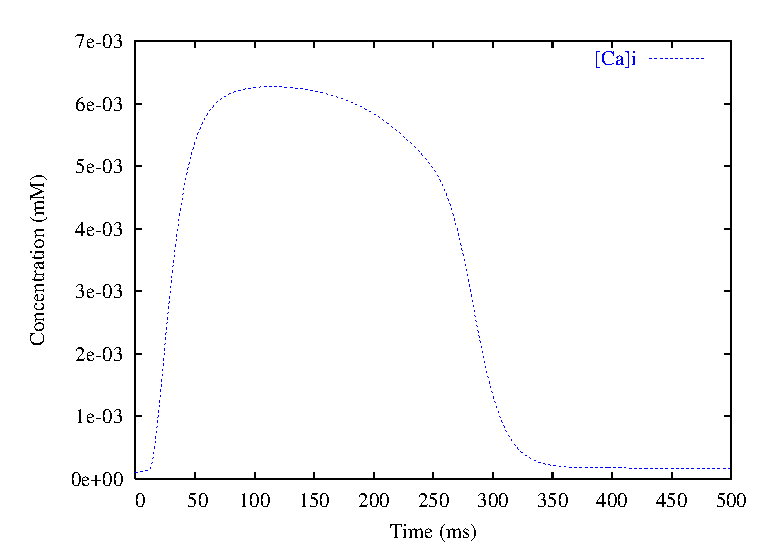
\includegraphics[width=75mm]{cardiac_electrophysiology/epsfiles/BRDR_Cai.eps}
  \caption[Defibrillation Beeler-Reuter intracellular calcium concentration]{The
    intracellular calcium ion concentration from the defibrillation Beeler-Reuter model.}
  \label{fig:BRDR_cai}
\end{figure}

In addition to these changes, in order to simulate ischemic tissue a scale
factor was added to the time dependent $d$ and $f$ gates to allow the scaling
of the action potential duration. The
modified equations became
\begin{align}
  \dby{d}{t}=&\dfrac{\alpha_{d}}{R}\cdot \pbrac{1-d}-\beta_{d}\cdot  d \\
  \dby{f}{t}=&\dfrac{\alpha_{f}}{R}\cdot \pbrac{1-f}-\beta_{f}\cdot  f
\end{align}
where $R$ was typically in the range of $1$ to $8$. 
The slow inward current and associated gating variables are shown in
\figref{fig:BRDR_Is_traces}.
\begin{figure}[hbtp] 
  \centering
  \begin{subfigure}[b]{0.45\linewidth}
    \centering
    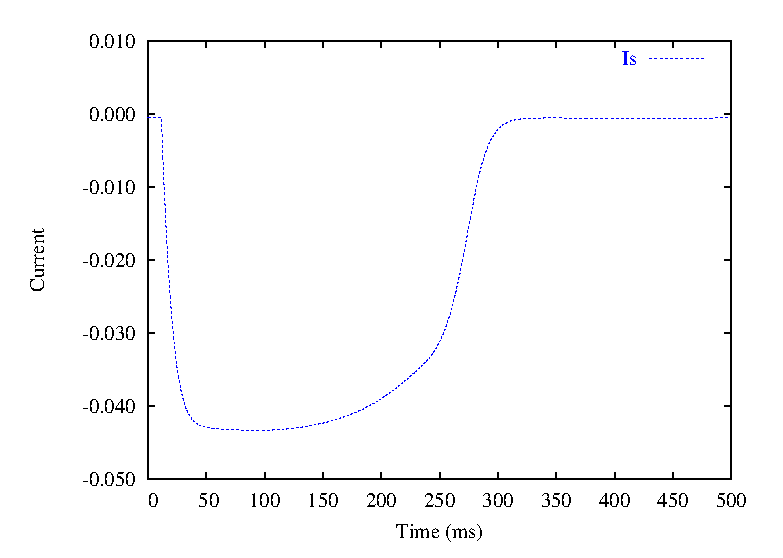
\includegraphics[width=\textwidth]{cardiac_electrophysiology/epsfiles/BRDR_Is.eps}
    \caption{}
  \end{subfigure}
  \hfill
  \begin{subfigure}[b]{0.45\linewidth}
    \centering
    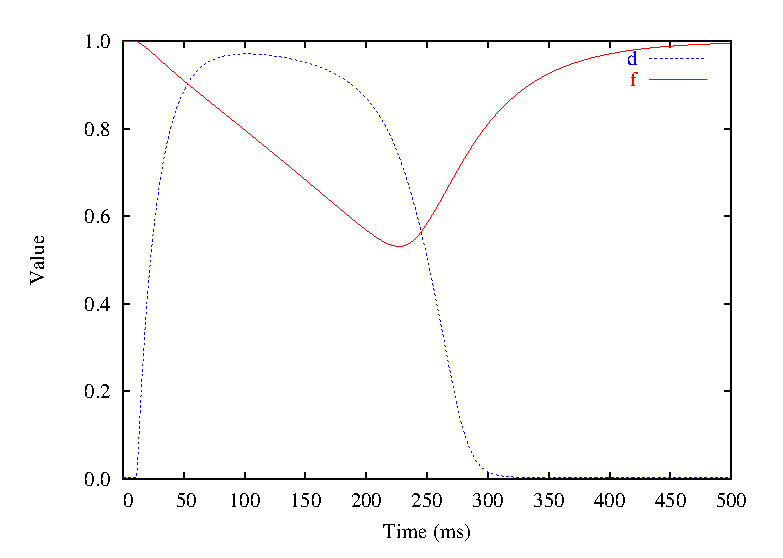
\includegraphics[width=\textwidth]{cardiac_electrophysiology/epsfiles/BRDR_df.eps}
    \caption{}
  \end{subfigure}
  \caption[Defibrillation Beeler-Reuter slow inward current]{Figure(a) shows the
    slow inward current over time and Figure(b) shows the
    $d$ and $f$ gate variables over time from the defibrillation Beeler-Reuter model.}
  \label{fig:BRDR_Is_traces}
\end{figure}
%
%===================================================================
\subsection{The Luo-Rudy models}
\label{sec:The_Luo-Rudy_I_model}
%===================================================================
The Luo-Rudy model \cite{luo:1991} built on the Beeler-Reuter model adjusting the
parameters to more recent experimental results and adding more currents to
more accurately represent the potassium ion dynamics. Six individual currents
were used to describe the cellular processes.
\begin{equation}
  I_{ion}=I_{Na}+I_{si}+I_{K}+I_{K1}+I_{Kp}+I_{b}
\end{equation}
Three of the currents may be grouped to give an expression for the total time
independent potassium current.
\begin{equation}
  I_{K1T}=I_{K1}+I_{Kp}+I_{b}
\end{equation}
A plot of $I_{K1T}$ is shown later in \figref{fig:LR_IbK1T_traces}. In
addition to these ionic currents the intracellular calcium ion
concentration was tracked due to the calcium uptake by the slow inward
current, $I_{si}$. The action potential produced by the Luo-Rudy model is
shown in \figref{fig:LR1_ap}.
\begin{figure}[hbtp] 
  \centering
  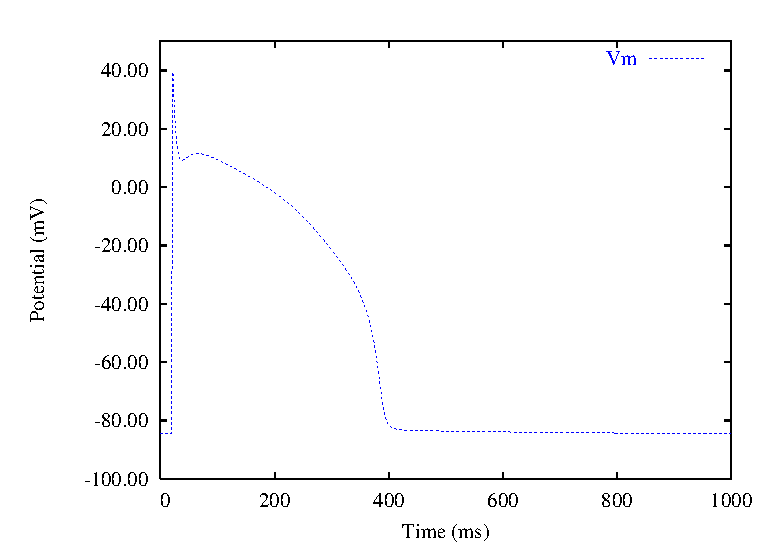
\includegraphics[width=75mm]{cardiac_electrophysiology/epsfiles/LR_Vm.eps}
  \caption[Luo-Rudy action potential]{Action potential trace from the Luo-Rudy
    ionic current model.}
  \label{fig:LR1_ap}
\end{figure}
%
\subsubsection{Fast inward sodium current}
The general form of the fast inward sodium current is the same as the original
Beeler-Reuter model with the omission of the steady state sodium conductance
parameter.
\begin{equation}
  I_{Na}=\overline{g_{Na}}\cdot m^3\cdot h\cdot j\cdot\pbrac{V_m-E_{Na}}
\end{equation}
Here $m$ is the activation gate, $h$ is the fast inactivation gate and $j$ is the slow
inactivation gate. The time dependent behaviour of these gates was identical to the
Beeler-Reuter model \eqnthrurefs{eqn:br_mt}{eqn:br_jt} but with reformulated
rate constants. $\overline{g_{Na}}$ is
the maximum sodium conductance and $E_{Na}$ is the reversal potential of the
channel as calculated from the Nernst potential for sodium ions using
\eqnref{eqn:lr1reversal}. The $\alpha$ and $\beta$ gating parameters were
defined to be
\begin{gather}
  \label{eqn:lr1_ina_coeffs}
  \begin{aligned}
    \alpha_m &= {0.32  (V_m+47.13) \over 1-\exp(-0.1(V_m+47.13))} \\
    \beta_m &= 0.08  \exp(-V_m / 11) \\
    \alpha_h &=
    \begin{cases}
      0 & \text{if $V_m \geq -40 \mV$} \\
      0.135  \exp[(-80.0-V_m) / 6.8] & \text{if $V_m < -40 \mV$}
    \end{cases} \\
    \beta_h &=
    \begin{cases}
      \frac{1}{0.13  (1 + \exp[- (V_m+10.66) / 11.1])} &
      \text{if $V_m \geq -40 \mV$} \\
      3.56  \exp(0.079 V_m) + \nttento{3.1}{5}  \exp(0.35  V_m) & 
      \text{if $V_m < -40 \mV$}
    \end{cases} \\
    \alpha_j &= 
    \begin{cases}
      0 & \text{if $V_m \geq -40 \mV$} \\
      \frac{\nttento{-1.2714}{5} \exp(0.2444 V_m) - \nttento{3.474}{-5} 
      \exp(-0.04391 V_m)}{1+\exp\left(0.311 (V_m+79.23) \right)} (V_m+37.78)&
      \text{if $V_m < -40 \mV$}
    \end{cases} \\
    \beta_j &=
    \begin{cases}
      0.3  \exp(\nttento{-2.535}{-7}  V_m) \over \left(1+\exp\left(-0.1 
          (V_m+32) \right) \right) & \text{if $V_m \geq -40 \mV$} \\
      0.1212  \exp( -0.01052  V_m) \over \left(1+\exp\left(-0.1378 
          (V_m+40.14) \right) \right)
      & \text{if $V_m < -40 \mV$}
    \end{cases}
  \end{aligned}
\end{gather}
The fast inward sodium current and the three gating variables are shown in
\figref{fig:LR_NA_traces}.
\begin{figure}[hbtp] 
  \centering
  \begin{subfigure}[b]{0.45\linewidth}
    \centering
    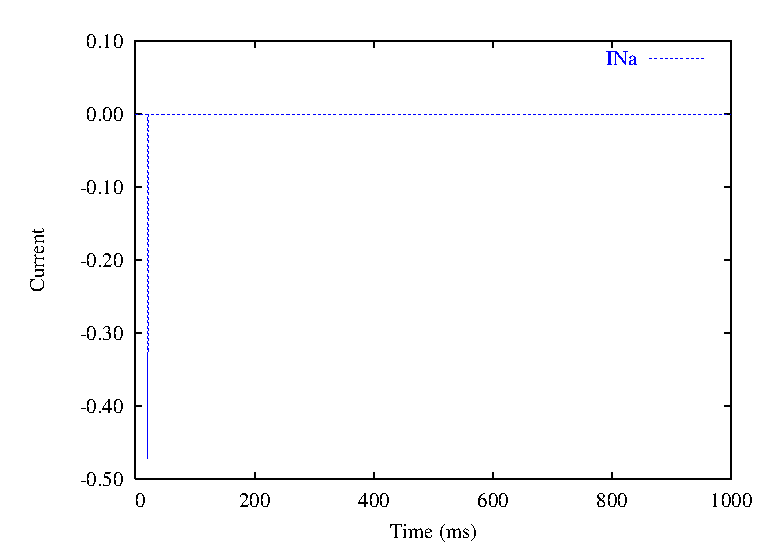
\includegraphics[width=\textwidth]{cardiac_electrophysiology/epsfiles/LR_INa.eps}
    \caption{}
  \end{subfigure}
  \hfill
  \begin{subfigure}[b]{0.45\linewidth}
    \centering
    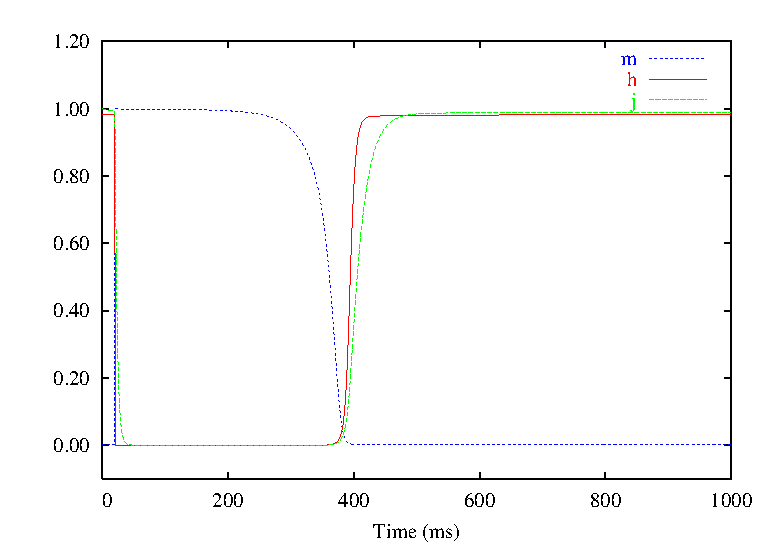
\includegraphics[width=\textwidth]{cardiac_electrophysiology/epsfiles/LR_NaGates.eps}
    \caption{}
  \end{subfigure}
  \caption[Fast inward sodium current from the Luo-Rudy model]{Figure(a) shows the
    fast inward sodium current over time and Figure(b) shows the $m$, $h$ and
    $j$ gate variables over time from the Luo-Rudy model.}
  \label{fig:LR_NA_traces}
\end{figure}
%
\subsubsection{Slow inward current}
The slow inward current was defined by the same formula as the $I_s$ current
in the Beeler Reuter model.
\begin{equation}
  I_{si}=\overline{g_{si}}\cdot d\cdot f\cdot \pbrac{V_m-E_{si}}
\end{equation}
The reversal potential was adjusted to be
\begin{equation}
  E_{si}=7.7-13.0287\ln\pbrac{\conc{Ca^{2+}}{i}}
\end{equation}
and the formulation of the rate constants, $\alpha_d$,$\beta_d$,$\alpha_f$
and $\beta_f$ were also unchanged. The current trace over time along with the
two gates are shown in \figref{fig:LR_Isi_traces}.
\begin{figure}[hbtp] 
  \centering
  \begin{subfigure}[b]{0.45\linewidth}
    \centering
    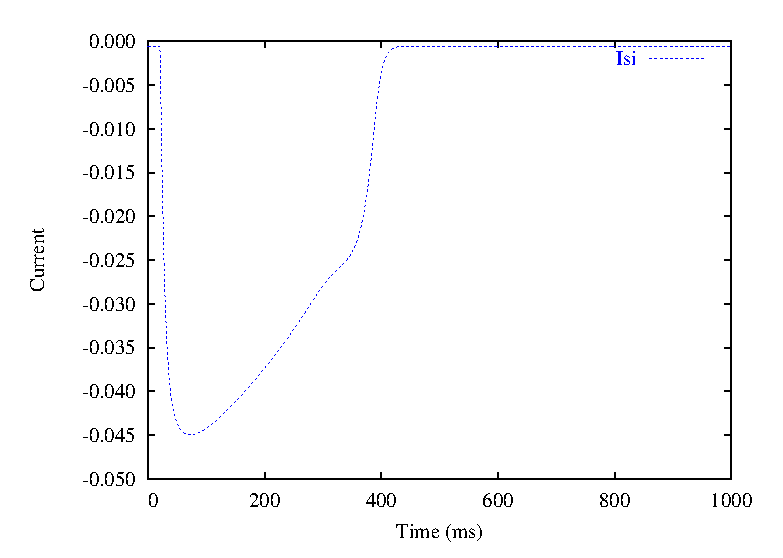
\includegraphics[width=\textwidth]{cardiac_electrophysiology/epsfiles/LR_Isi.eps}
    \caption{}
  \end{subfigure}
  \hfill
  \begin{subfigure}[b]{0.45\linewidth}
    \centering
    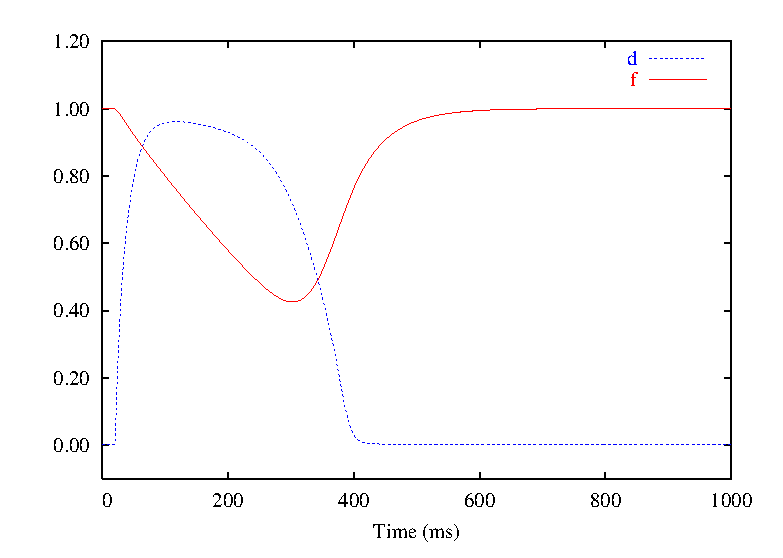
\includegraphics[width=\textwidth]{cardiac_electrophysiology/epsfiles/LR_SIGates.eps}
    \caption{}
  \end{subfigure}
  \caption[Slow inward current from the Luo-Rudy model]{Figure(a) shows the
    slow inward current over time and Figure(b) shows the $d$ and
    $f$ gate variables over time from the Luo-Rudy model.}
  \label{fig:LR_Isi_traces}
\end{figure}
%
\subsubsection{Time dependent potassium current}
The time dependent potassium current was controlled by an activation gate, $x$
and an inactivation gate, $X_i$. The inactivation gate was not formulated as a
typical Hodgkin-Huxley differential equation. 
\begin{equation}
  I_K=\overline{g_{K}}\cdot x\cdot X_i\cdot \pbrac{V_m-E_{K}}
\end{equation}
where the maximum potassium conductance was calculated from
\begin{equation}
  \overline{g_{K}}=g_{K}\cdot \sqrt{\conc{K^+}{o}/5.4}
\end{equation}
The reversal potential was calculated from
\begin{equation}
  E_K=\dfrac{RT}{F}\ln\pbrac{\dfrac{\conc{K^+}{o}+PR_{NaK}
      \conc{Na^+}{o}}{\conc{K^+}{i}+PR_{NaK}\conc{Na^+}{i}}}
\end{equation}
where $PR_{NaK}$ is a dimensionless permeability ratio. The rate constants
for the $x$ gate were 
defined to be the same as in the Beeler-Reuter model where the gate is
referenced as the $x1$ gate. This model introduces a new inactivation gate,
$X_i$, which was given by
\begin{gather}
  \begin{aligned}
    X_i &=
    \begin{cases}
      1.0 & \text{if $V_m \leq -100 \mV$} \\
      2.837 \dfrac{\exp\pbrac{0.04\pbrac{V_m+77}}-1}{\pbrac{V_m+77}
        \exp\pbrac{0.04\pbrac{V_m+35}}} & \text{otherwise}
    \end{cases} \\ 
  \end{aligned}
\end{gather}
The temporal trace of the time dependent potassium current along with the $x$
gating variable is shown in \figref{fig:LR_IK_traces}.
\begin{figure}[hbtp] 
  \centering
  \begin{subfigure}[b]{0.45\linewidth}
    \centering
    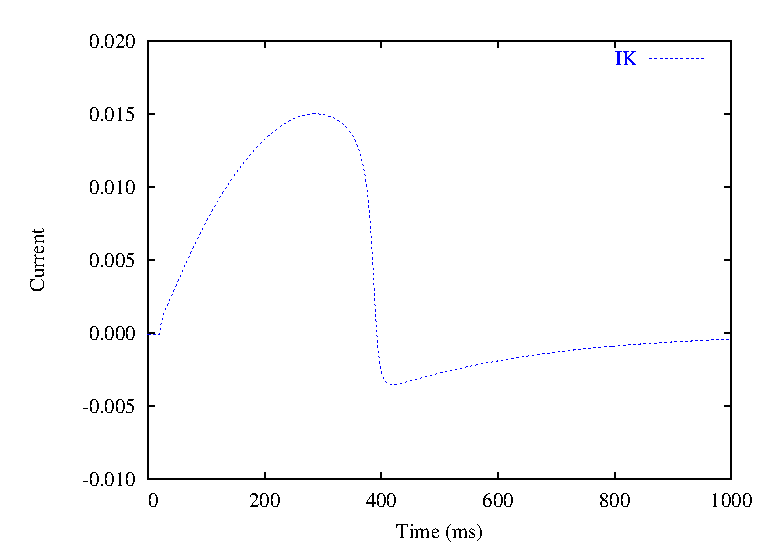
\includegraphics[width=\textwidth]{cardiac_electrophysiology/epsfiles/LR_IK.eps}
    \caption{}
  \end{subfigure}
  \hfill
  \begin{subfigure}[b]{0.45\linewidth}
    \centering
    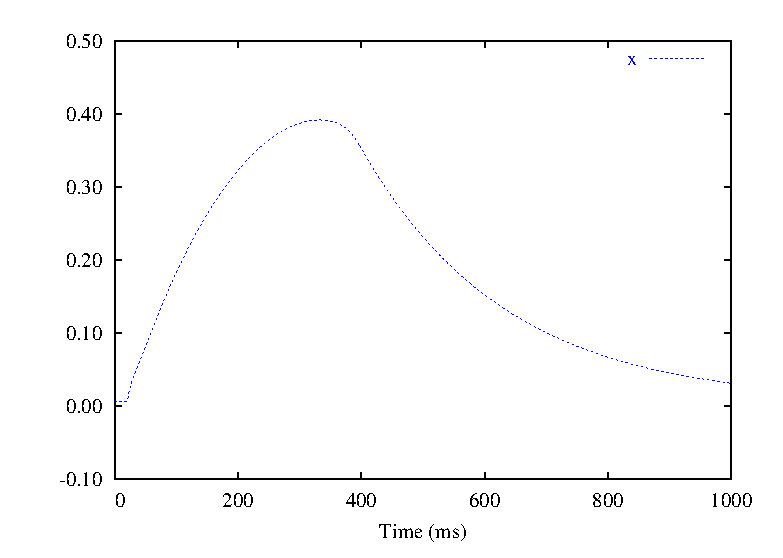
\includegraphics[width=\textwidth]{cardiac_electrophysiology/epsfiles/LR_Xgate.eps}
    \caption{}
  \end{subfigure}
  \caption[Time dependent outward current from the Luo-Rudy model]{Figure(a) shows the
    time dependent outward current over time and Figure(b) shows the $x$ gate
    over time from the Luo-Rudy model.}
  \label{fig:LR_IK_traces}
\end{figure}
%
\subsubsection{Time independent potassium current}
While present in the Beeler-Reuter model the time independent potassium
current has been formulated differently along with the addition of two further
potassium based time independent currents, $I_{Kp}$ and $I_b$. This model uses
one gating variable with a time constant small enough that it may be
approximated by a steady state formulation.
\begin{equation}
  I_{K1}=\overline{g_{K1}}\cdot K_{1\infty}\cdot \pbrac{V_m-E_{K1}}
\end{equation}
The reversal potential was the Nernst potential for potassium ions found from
\eqnref{eqn:lr1reversal}. The maximum channel conductance was calculated by
\begin{equation}
  \overline{g_{K1}}=g_{K1}\cdot \sqrt{\conc{K^+}{o}/5.4}
\end{equation}
The steady gating parameter, $K_{1\infty}$ was calculated to be
\begin{equation}
  K_{1\infty}=\dfrac{\alpha_{K1}}{\alpha_{K1}+\beta{K1}}
\end{equation}
where the rate constants were given by
\begin{align}
  \alpha_{K1}=& \dfrac{1.02}{1+\exp\sqbrac{0.2385\pbrac{V_m-E_{K1}-59.215}}} \\
  \beta_{K1}=& \dfrac{{0.49124\exp\sqbrac{0.08032\pbrac{V_m-E_{K1}+5.476}}}+
    {\exp\sqbrac{0.06175\pbrac{V_m-E_{K1}-594.31}}}}{1+\exp\sqbrac{-0.5143
    \pbrac{V_m-E_{K1}+4.753}}}
\end{align}
A plot of the time independent potassium current is shown in \figref{fig:LR_IK1p_traces}.
%
\subsubsection{Plateau potassium current}
The reversal potential for the plateau potassium current was the same as the
reversal potential of the time independent potassium current.
\begin{equation}
  E_{Kp}=E_{K1}
\end{equation}
The ionic current was given by
\begin{equation}
 I_{Kp}=\overline{g_{Kp}}\cdot K_p\cdot \pbrac{V_m-E_{Kp}}
\end{equation}
where
\begin{equation}
  K_p=\dfrac{1}{1+\exp\pbrac{\pbrac{7.488-V_m}/5.98}}
\end{equation}
A plot of the plateau potassium current is shown in \figref{fig:LR_IK1p_traces}.
\begin{figure}[hbtp] 
  \centering
  \begin{subfigure}[b]{0.45\linewidth}
    \centering
    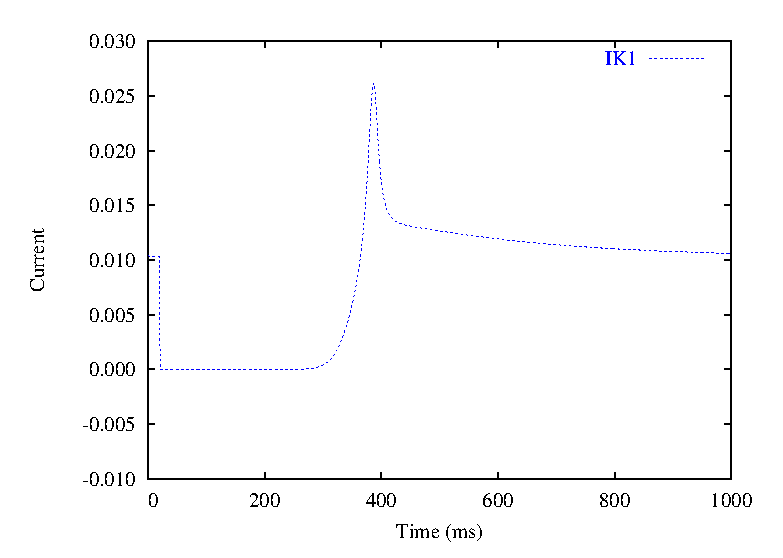
\includegraphics[width=\textwidth]{cardiac_electrophysiology/epsfiles/LR_IK1.eps}
    \caption{}
  \end{subfigure}
  \hfill
  \begin{subfigure}[b]{0.45\linewidth}
    \centering
    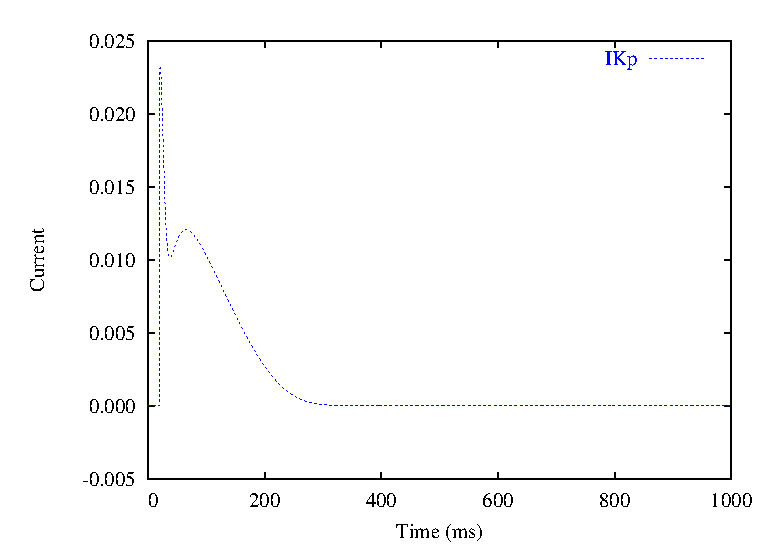
\includegraphics[width=\textwidth]{cardiac_electrophysiology/epsfiles/LR_IKp.eps}
    \caption{}
  \end{subfigure}
  \caption[Time independent and plateau currents from the Luo-Rudy model]{Figure(a) shows the
    time independent outward current over time and Figure(b) shows the plateau
    current over timefrom the Luo-Rudy model.}
  \label{fig:LR_IK1p_traces}
\end{figure}
%
\subsubsection{Background current}
The background current was given by
\begin{equation}
  I_b=\overline{g_{b}}\cdot \pbrac{V_m+59.87}
\end{equation}
and a plot of the background current over time is shown in \figref{fig:LR_IbK1T_traces}.
\begin{figure}[hbtp] 
  \centering
  \begin{subfigure}[b]{0.45\linewidth}
    \centering
    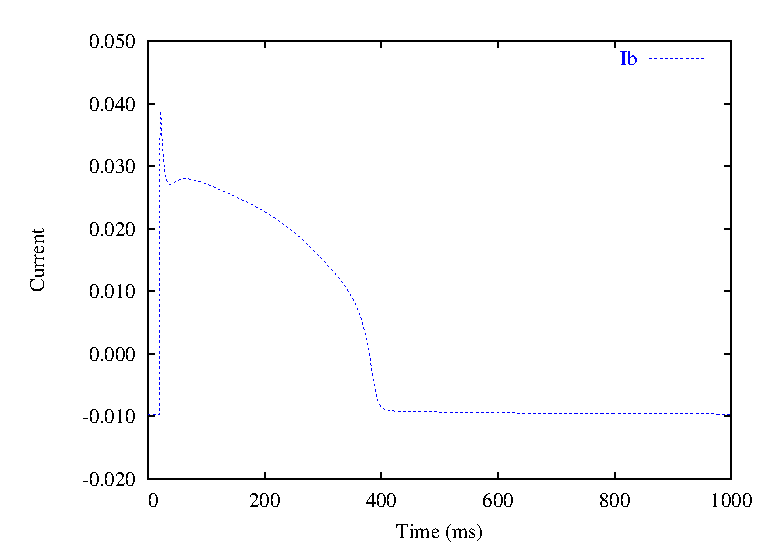
\includegraphics[width=\textwidth]{cardiac_electrophysiology/epsfiles/LR_Ib.eps}
    \caption{}
  \end{subfigure}
  \hfill
  \begin{subfigure}[b]{0.45\linewidth}
    \centering
    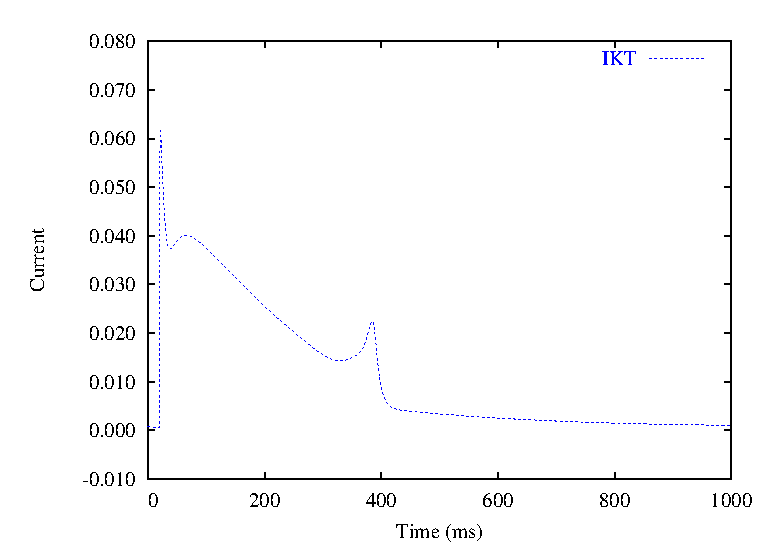
\includegraphics[width=\textwidth]{cardiac_electrophysiology/epsfiles/LR_IKT.eps}
    \caption{}
  \end{subfigure}
  \caption[Background and total time independent currents from the Luo-Rudy
  model]{Figure(a) shows the 
    background current over time and Figure(b) shows the total time
    independent potassium current over time from the Luo-Rudy model.}
  \label{fig:LR_IbK1T_traces}
\end{figure}
%
\subsubsection{Model parameters}
The set of model parameters in consistent units used with the Luo-Rudy model
are given in this section. The initial value of the transmembrane potential
was set to be $-84.5\mV$. The initial values of the gating variables which
were also time dependent are shown in \tabref{tab:lr1_init_gates}.
\begin{table}[hbtp] \centering
  \begin{tabular}{|c|c|}
    \hline
    \emph{Gate} & \emph{Initial value} \\ 
    \hline
    \hline 
      $m$ & $1.67 \times 10^{-3}$ \\
      $h$ & $9.38 \times 10^{-1}$ \\
      $j$ & $1.0$ \\
      $d$ & $2.98 \times 10^{-3}$ \\
      $f$ & $1.0$ \\
      $x$ & $6.02 \times 10^{-3}$ \\
    \hline
  \end{tabular}
  \caption[Initial gate values for the Luo-Rudy I model]{Initial gate
    values for the Luo-Rudy I model}
  \label{tab:lr1_init_gates}
\end{table}
The other time dependent quantity is the intracellular calcium
concentration. All of the other concentrations were constant over time. 
The intracellular and extracellular ion concentrations for the three
ions included in the model are shown in \tabref{tab:lr1_init_ions}.
\begin{table}[hbtp] \centering
  \begin{tabular}{|c|c|}
    \hline
    \emph{Ion} & \emph{Initial value} \\ 
    \hline
    \hline 
      $\conc{Ca^{2+}}{i}$ & $1.78 \times 10^{-4}$ \\
      $\conc{Ca^{2+}}{o}$ & $1.8$ \\
      $\conc{K^{+}}{i}$ & $1.45 \times 10^{2}$ \\
      $\conc{K^{+}}{o}$ & $5.4$ \\
      $\conc{Na^{+}}{i}$ & $1.8 \times 10^{1}$ \\
      $\conc{Na^{+}}{o}$ & $1.4 \times 10^{2}$ \\
    \hline
  \end{tabular}
  \caption[Initial ion concentrations for the Luo-Rudy I model]{Initial ion
    concentrations for the Luo-Rudy I model}
  \label{tab:lr1_init_ions}
\end{table}
All concentrations are given in $\nM\unitseparator\mm^{-3}=\mM$. Where in the
Beeler-Reuter model the reversal potentials of a given channel were
directly set, in this model they were calculated from the ion concentrations. The
reversal potential of a particular ion $x$ was defined by its Nernst potential to be 
\begin{equation}
  E_{x}=\pbrac{\dfrac{RT}{z_xF}}\ln{\dfrac{\conc{x}{o}}{\conc{x}{i}}}
  \label{eqn:lr1reversal}
\end{equation}
where $R$ is the gas constant, $T$ is temperature, $F$ is Faradays constant
$z_x$ is the valence of ion $x$ and $\conc{x}{o}$,$\conc{x}{i}$ were the
extracellular and intracellular 
concentrations of ion $x$ respectively. The maximum conductance values used
are shown in \tabref{tab:lr1_conductance}.  
\begin{table}[hbtp] \centering
  \begin{tabular}{|c|c|}
    \hline
    \emph{Parameter} & \emph{Value} \\ 
    \hline
    \hline 
      $\overline{g_{Na}}$ & $2.3 \times 10^{-1}$ \\
      $\overline{g_{si}}$ & $9.0 \times 10^{-4}$ \\
      $g_{K}$ & $2.82 \times 10^{-3}$ \\
      $g_{K1}$ & $6.047 \times 10^{-3}$ \\
      $\overline{g_{Kp}}$ & $1.83 \times 10^{-4}$ \\
      $\overline{g_{b}}$ & $3.921 \times 10^{-4}$ \\
    \hline
  \end{tabular}
  \caption[Conductance values for the Luo-Rudy I model]{Conductance
    values for the Luo-Rudy I model}
  \label{tab:lr1_conductance}
\end{table}
All conductances are given in $\mS\unitseparator\mm^{-2}$. It should be noted
that the maximum conductances for $g_{K}$ and $g_{K1}$ are calculated
elsewhere in the model using these values. The values for the other parameters
used in the model are shown in \tabref{tab:lr1_params}. Here $C_m$ is the
membrane capacitance and $A_m$ is the surface to volume 
ratio. 
\begin{table}[hbtp] \centering
  \begin{tabular}{|c|c|c|}
    \hline
    \emph{Parameter} & \emph{Value} & \emph{Units}\\ 
    \hline
    \hline 
      $C_m$ & $1.0 \times 10^{-2}$ & $\uF\unitseparator\mm^{-2}$ \\
      $A_m$ & $1.0 \times 10^{2}$  & $\pmm$ \\
      $R$ & $8.314472 \times 10^{3}$ & $\pJ\unitseparator
      \nM^{-1}\unitseparator \degK^{-1}$ \\
      $T$ & $3.1 \times 10^{2}$ & $\degK$\\
      $F$ & $9.648534 \times 10^{4}$ & $\nC\unitseparator\nM^{-1}$ \\
      $PR_{NaK}$ & $1.833 \times 10^{-2}$ & $dimensionless$ \\
    \hline
  \end{tabular}
  \caption[Parameter values for the Luo-Rudy I model]{Parameter
    values for the Luo-Rudy I model}
  \label{tab:lr1_params}
\end{table}
%
%===================================================================
%\subsection{The Luo-Rudy II model}
%\label{sec:The_Luo-Rudy_II_model}
%===================================================================
\subsubsection{The Luo-Rudy II model}
The second model published by Luo and Rudy \cite{luo:1994a} has become a widely used
model in the field of cellular cardiac activation and while designed
for mammalian ventricular cells was based mainly on the guinea pig. Again the
units of the model parameters where adjusted to retain unit consistency. One
of the main features of the model was the inclusion of more detailed calcium
dynamics. The model used $15$ ionic currents to generate action potentials.
\begin{align}
  I_{ion} =&
  I_{Na}+I_{Ca\pbrac{L}}+I_{K}+I_{K1}+I_{Kp}+I_{NaCa}+I_{NaK}+I_{ns\pbrac{Ca}}\nonumber\\
  +& I_{p\pbrac{Ca}}+I_{Ca,b}+I_{Na,b}+I_{rel}+I_{up}+I_{leak}+I_{tr}
\end{align}
%
\subsubsection{Initial ion concentrations}
The initial intracellular and extracellular ion concentrations for the three
ions included in the model are shown in \tabref{tab:lr2_init_ions}.
\begin{table}[hbtp] \centering
  \begin{tabular}{|c|c|}
    \hline
    \emph{Ion} & \emph{Initial value} \\ 
    \hline
    \hline 
      $\conc{Ca^{2+}}{i}$ & $1.2 \times 10^{-4}$ \\
      $\conc{Ca^{2+}}{o}$ & $1.8$ \\
      $\conc{K^{+}}{i}$ & $1.45 \times 10^{2}$ \\
      $\conc{K^{+}}{o}$ & $5.4$ \\
      $\conc{Na^{+}}{i}$ & $1.0 \times 10^{1}$ \\
      $\conc{Na^{+}}{o}$ & $1.4 \times 10^{2}$ \\
    \hline
  \end{tabular}
  \caption[Initial ion concentrations for the Luo-Rudy II model]{Initial ion
    concentrations for the Luo-Rudy II model}
  \label{tab:lr2_init_ions}
\end{table}
All concentrations are given in $\nM\unitseparator\mm^{-3}=\mM$.
%Where in the Beeler-Reuter model the reversal potentials of a channel were
%directly set, in this model they are calculated from ion concentrations.
As is the case with the Luo-Rudy I model, the reversal potential of
a particular ion $x$ is defined by \eqnref{eqn:lr1reversal}.
%\begin{equation}
%  E_{x}=\pbrac{\dfrac{RT}{z_x F}}\ln{\dfrac{\conc{x}{o}}{\conc{x}{i}}}
%  \label{eqn:lr2reversal}
%\end{equation}
%where $R$ is the gas constant which was set to $8314.472~pJ\unitseparator
%\nM^{-1}\unitseparator K^{-1}$, $T$ is the temperaturewhich was set to be
%$310~K$, $F$ is Faradays constant which was $96485.341~nC\unitseparator
%\nM^{-1}$ and $\conc{x}{o}$,$\conc{x}{i}$ were the extracellular and
%intracellular concentrations of ion $x$ respectively.
%
\subsubsection{Fast inward sodium current}
The general form of the fast inward sodium current is the same as the original
Luo-Rudy model.
\begin{equation}
  I_{Na}=\overline{g_{Na}}m^3hj\pbrac{V_m-E_{Na}}
\end{equation}
Here $m$ is the activation gate, $h$ is the inactivation gate and $j$ is the slow
inactivation gate. The time dependence of these gates was identical to the
Beeler-Reuter model \eqnthrurefs{eqn:br_mt}{eqn:br_jt}. $\overline{g}_{Na}$ is
the maximum sodium conductance which was set to be $1.6 \times 10^{-1}
\mS\unitseparator\mm^{-2}$ and $E_{Na}$ is the reversal potential of the
channel which was calculated from the sodium ion concentration using
\eqnref{eqn:lr1reversal}. The $\alpha$ and $\beta$ gating parameters were
defined to be
\begin{gather}
  \label{eqn:lr2_ina_coeffs}%\renewcommand{\arraystretch}{1.75}
  \begin{aligned}
    \alpha_m &= {0.32  (V_m+47.13) \over 1-\exp(-0.1(V_m+47.13))} \\
    \beta_m &= 0.08  \exp(-V_m / 11) \\
    \alpha_h &=
    \begin{cases}
      0 & \text{if $V_m \geq -40 \mV$} \\
      0.135  \exp[(-80.0-V_m) / 6.8] & \text{if $V_m < -40 \mV$}
    \end{cases} \\
    %\renewcommand{\arraystretch}{2.5}
    \beta_h &=
    \begin{cases}
      \frac{1}{0.13  (1 + \exp[- (V_m+10.66) / 11.1])} &
      \text{if $V_m \geq -40 \mV$} \\
      3.56  \exp(0.079 V_m) + \nttento{3.1}{5}  \exp(0.35  V_m) & 
      \text{if $V_m < -40 \mV$}
    \end{cases} \\
    \alpha_j &= 
    \begin{cases}%\renewcommand{\arraystretch}{1.5}
      0 & \text{if $V_m \geq -40 \mV$} \\
      \frac{\nttento{-1.2714}{5} \exp(0.2444 V_m) - \nttento{3.474}{-5} 
      \exp(-0.04391 V_m)}{1+\exp\left(0.311 (V_m+79.23) \right)} (V_m+37.78)&
      \text{if $V_m < -40 \mV$}
    \end{cases} \\
    \beta_j &=
    \begin{cases}%\renewcommand{\arraystretch}{1.5}
      0.3  \exp(\nttento{-2.535}{-7}  V_m) \over \left(1+\exp\left(-0.1 
          (V_m+32) \right) \right) & \text{if $V_m \geq -40 \mV$} \\
      0.1212  \exp( -0.01052  V_m) \over \left(1+\exp\left(-0.1378 
          (V_m+40.14) \right) \right)
      & \text{if $V_m < -40 \mV$}
    \end{cases}
  \end{aligned}
\end{gather}
%
\subsubsection{L-type calcium currents}
The current associated with the L-type calcium channel was divided into three
separate currents for the three ions which pass through the channel.
\begin{equation}
  I_{Ca\pbrac{L}}=I_{Ca\pbrac{L},Ca}+I_{Ca\pbrac{L},Na}+I_{Ca\pbrac{L},K}
\end{equation}
where
\begin{align}
  I_{Ca\pbrac{L},Ca}&=dff_{Ca}\overline{I_{Ca\pbrac{L},Ca}} \\
  I_{Ca\pbrac{L},Na}&=dff_{Ca}\overline{I_{Ca\pbrac{L},Na}} \\
  I_{Ca\pbrac{L},K}&=dff_{Ca}\overline{I_{Ca\pbrac{L},K}} 
\end{align}
The activation gate, $d$ and the inactivation gate, $f$ are controlled by
Hodgkin-Huxley type differential equations \eqnrefs{eqn:br_dt}{eqn:br_ft} and
a further inactivation gate, $f_{Ca}$ is governed by the following equation.
\begin{equation}
  f_{Ca}=\dfrac{1}{1+\pbrac{\dfrac{\conc{Ca^{2+}}{i}}{K_{m,Ca}}}^2}
\end{equation}
where $K_{m,Ca}$ is the half activation concentration for $Ca^{2+}$ which was
set to be $6.0 \times 10^{-4} \mM$. The rate constants for the $d$ and $f$
gates were defined to be
\begin{align}
  \alpha_d=& d_{\infty}/\tau_d \\
  \beta_d=& \pbrac{1-d_{\infty}}/\tau_d\\
  \alpha_f=&f_{\infty}/\tau_f \\
  \beta_f=& \pbrac{1-f_{\infty}}/\tau_f
\end{align}
where
\begin{align}
  d_{\infty} &= \frac{1}{1 + \exp \left(-\frac{V_m +
  10}{6.24}\right)}\\ 
  \tau_d &= d_{\infty} \frac{1-\exp
  \left(-\frac{V_m+10}{6.24}\right)}{0.035 \left(V_m+10\right)}
\end{align}
and
\begin{align}
  f_{\infty} &= \frac{1}{1+\exp \left(\frac{V_m+35.06}{8.6}\right)} +
  \frac{0.6}{1+\exp \left(\frac{50-V_m}{20}\right)} \\
  \tau_f &= \frac{1}{0.0197 \exp \left( -\left[0.0337 \left( V_m + 10
  \right)\right]^2 \right) + 0.02}
\end{align}
The three fully activated current terms, $\overline{I_{Ca\pbrac{L},x}}$ were
calculated from 
\begin{equation}
  \label{eqn:lr2_ical_fullyact}
   \overline{I_{Ca\pbrac{L},x}}= P_{x}z_{x}^2\dfrac{V_m F^2}{R T}
  \dfrac{\gamma_{xi}\conc{x}{i}\exp \left(z_{x} V_m F / R
  T\right) - \gamma_{xo} \conc{x}{o}}{\exp \left(z_{x} V_m F / R
  T\right) - 1}
\end{equation}
where the $Ca^{2+}$, $Na^+$ and $K^+$ ions are substituted for $x$ where
appropriate. $P_x$ is the permeability of the membrane to ion $x$, $z_x$ is
the valence of ion $x$ and $\gamma_{xi}$,$\gamma_{xo}$ are the intracellular
and extracellular activity coefficients of ion
$x$. \Tabref{tab:lr2_lca_constants} shows the 
coefficients which were used for each ion.
\begin{table}[hbtp] \centering
  \begin{tabular}{|c|c|}
    \hline
    \emph{Quantity} & \emph{Value} \\ 
    \hline
    \hline 
      $P_{Ca}$ & $5.4 \times 10^{-6} \mm\unitseparator\ms^{-1}$ \\
      $P_{Na}$ & $6.75 \times 10^{-9}\mm\unitseparator\ms^{-1}$ \\
      $P_{K}$ & $1.93 \times 10^{-9}\mm\unitseparator\ms^{-1}$ \\
      $\gamma_{Cai}$ & $1.0$ \\
      $\gamma_{Nai}$ & $7.5 \times 10^{-1}$ \\
      $\gamma_{Ki}$ & $7.5 \times 10^{-1}$ \\
      $\gamma_{Cao}$ & $3.41 \times 10^{-1}$ \\
      $\gamma_{Nao}$ & $7.5 \times 10^{-1}$ \\
      $\gamma_{Ko}$ & $7.5 \times 10^{-1}$ \\
    \hline
  \end{tabular}
  \caption[L-type calcium channel constants]{L-type calcium channel constants}
  \label{tab:lr2_lca_constants}
\end{table}
%
\subsubsection{Time independent potassium current}
This current features a single squared activation gate, $X$ and a
time independent inactivation gate $X_i$. The current is formulated to be
\begin{equation}
  I_K = \overline{g}_{K}X_iX^2\pbrac{V_m-E_K}
\end{equation}
where $\overline{g}_{K}$ was  set to be
\begin{equation}
  \overline{g}_{K}=0.00282\sqrt{\dfrac{\conc{K^+}{o}}{5.4}}
\end{equation}
and the reversal potential, $E_K$ was
\begin{equation}
  E_K =
  \dfrac{RT}{F}\ln\pbrac{\dfrac{\conc{K^+}{o}+P_{NaK}\conc{Na^+}{o}}
  {\conc{K^+}{i}+P_{NaK}\conc{Na^+}{i}}}
\end{equation}
where $P_{NaK}$ is the $Na$/$K$ permeability ratio and was set to be $1.833
\times 10^{-2} (dimensionless)$. The gating variable $X$ is governed by a
standard Hogkin-Huxley differential equation.
\begin{gather}
  \label{eqn:lr2_ik_coeffs}
  \begin{aligned}
    \alpha_X &= \dfrac{7.19\times 10^{-5} \pbrac{V_m + 30}}{1 - \exp
      \pbrac{-0.148
     \pbrac{V_m + 30}}} \\
    \beta_X &= \dfrac{1.31\times 10^{-4} \pbrac{V_m + 30}}{-1 + \exp \pbrac{0.0687
     \pbrac{V_m + 30}}}
  \end{aligned}
\end{gather}
The time independent inactivation gate was calculated to be
\begin{equation}
  \label{eqn:lr2_ik_xi}
  X_i = \dfrac{1}{1 + \exp \left( \dfrac{V_m - 56.26}{32.1} \right)}
\end{equation}
%
\subsubsection{Time independent potassium current}
This channel contains a single inactivation gate whose time constant is small
enough that it may be approximated as steady state.
\begin{equation}
  \overline{g}_{K1} = 0.0075\sqrt{\dfrac{\conc{K^+}{o}}{5.4}}
\end{equation}

%===================================================================
\subsection{The Noble 98 model}
\label{sec:The_Noble_98_model}
%===================================================================
One of the features of this model is that it
was designed with a mind to incorporating other processes such as
mechanics,metabolism, pH dependence and drug receptor interactions. This model was also
designed to be solved rapidly allowing it to be used in large scale tissue simulations.
The model incorporates subspaces within the cell. These are the sarcoplasmic
reticulum (SR) which was divided into two parts, the network SR (NSR) and the
junctional SR (JSR), and a diadic space (DS) which lies between the JSR and
the T-tubules of the cell.
The ionic current term is made up of $27$ individual currents.
\begin{align}
  I_{ion}=&I_{K1}+I_{to}+I_{Kr1}+I_{Kr2}+I_{Ks}+I_{K,Na}+I_{b,K}+I_{K,ATP}+I_{K,ACh} \nonumber \\ 
         +&I_{Na}+I_{b,Na}+I_{p,Na}+I_{CaL,K}+I_{CaL,Na}+I_{CaL,Ca}+I_{Cal,KDS}+I_{CaL,NaDS}\nonumber \\ 
         +&I_{CaL,CaDS}+I_{b,Ca}+I_{NaK}+I_{NaCa}+I_{NaCaDS}+I_{K,stretch}+I_{Na,stretch} \nonumber \\
         +&I_{Ca,stretch}+I_{Ns,stretch}+I_{An,stretch}
\end{align}
%A brief description of the currents is given in \tabref{}.
%There are also four internal fluxes which are used to describe current flows
%within the cell which have time dependent properties. These fluxes are shown
%in \tabref{}.
%
%
%===================================================================
\section{Simplified models of cardiac cells}
\label{sec:Simplified_models_of_cardiac_cells}
%===================================================================
Often it is not necessary to model the ionic currents of a cell with the
accuracy and complexity inherent in the biophysically based models. With a view
to investigating phenomena on a larger spatial and temporal scale several
ionic current models have been developed which do not seek to model
subcellular processes but only to provide an action potential with minimal
computational cost. The simplest of these models is a polynomial model with
just one variable.
%
%===================================================================
\subsection{The polyomial model}
\label{sec:The_polynomial_model}
%===================================================================
The most common polynomial model used to describe activation processes is a
cubic polynomial model developed by \citeasnoun{hunter:1975} as shown in
\eqnref{eqn:cubic_ionic_current_model}. Because there is only a single
variable the model is very fast to compute so may be used on large geometries.
The cubic model generates cellular depolarisation but it does not attempt to
model repolarisation making it unsuitable for modelling any reentrant
phenomena. It is possible to generate an analytic solution for the conduction
velocity of the cubic model along a one dimensional fibre. The cubic ionic current
model is defined to be
\begin{equation}
  I_{ion} = g \sqbrac{ V_m \pbrac{ 1 - \dfrac{V_m}{V_{th}}}
  \pbrac{ 1 - \dfrac{V_m}{V_p}}}
  \label{eqn:cubic_ionic_current_model}
\end{equation}
where all potentials are expressed as deviations from a resting potential
$V_r$. $V_m$ is the transmembrane potential, $V_{th}$ is the threshold
potential, $V_p$ is the plateau potential and $g$ is the membrane conductance.
Typical values for these parameters are given in \tabref{tab:Cubic_Model_Params}.
\begin{table}[hbtp] \centering
  \begin{tabular}{|c|c|c|}
    \hline
    \emph{Parameter} & \emph{Units} & \emph{Value} \\ 
    \hline
    \hline 
    $V_r$ & $\mV$ & $-85.0$ \\
    $V_{th}$ & $\mV$ & $-75.0$ \\
    $V_p$ & $\mV$ & $-15.0$ \\
    $g$ & ${\mS\unitseparator\mm^{-2}}$ & $0.004$ \\
    $C_m$ & $\uF\unitseparator\mm^{-2}$ & $0.01$ \\
    $A_m$ & $\mm^{-1}$ & $200$ \\
    \hline
  \end{tabular}
  \caption[Typical parameters for the cubic ionic current model]{Typical
    parameters for the cubic ionic current model}
  \label{tab:Cubic_Model_Params}
\end{table}
The cubic model may be extended to a higher order polynomial ($5th$, $7th$
etc.) using the following formula to generate different depolarisation
profiles
\begin{equation}
  I_{ion} = g \sqbrac{ V_m \pbrac{ 1 - \pbrac{\dfrac{V_m}{V_{th}}}^n}
  \pbrac{ 1 - \pbrac{\dfrac{V_m}{V_p}}^n}}
  \label{eqn:cubic_ionic_current_model2}
\end{equation}
where $n$ is a positive integer. The activation profile generated using the
cubic ionic current model is shown in \figref{fig:cubic_cell_traces}.
\begin{figure}[hbtp] 
  \centering
  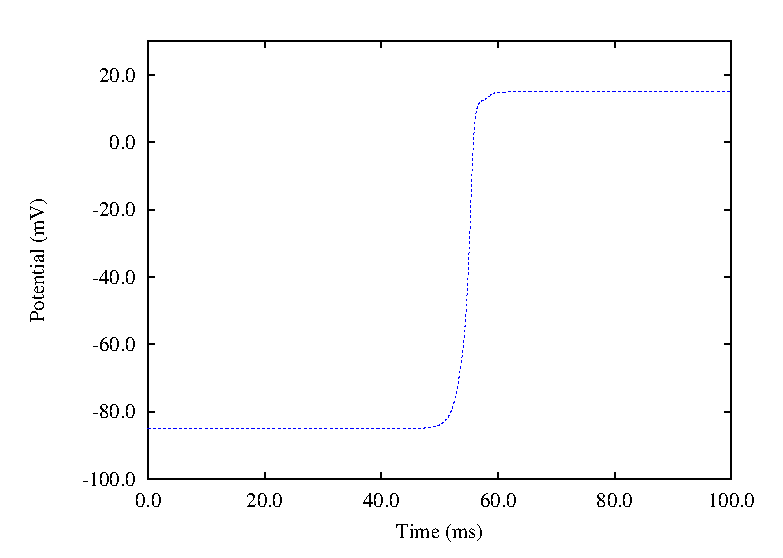
\includegraphics[width=75mm]{cardiac_electrophysiology/epsfiles/CubicVm.eps}
  \caption[Potential trace from a single cell using the cubic ionic current
  model]{Potential trace from a single cell using the cubic ionic current
    model}
  \label{fig:cubic_cell_traces}
\end{figure}
The polynomial models have roots at $V_r$, $V_{th}$ and $V_p$ causing any
stimulus under $V_{th}$ to return to rest and any suprathreshold stimulus to
move to the plateau potential $V_p$.
%
%===================================================================
\subsection{The FitzHugh-Nagumo model}
\label{The_FitzHugh-Nagumo_Model}
%===================================================================
The FitzHugh-Nagumo model is based on the cubic excitation model but also includes a recovery
variable so both depolarisation and repolarisation may be modelled. The form
of the model used was adapted from \citeasnoun{rogers:1994a}. The model
normalises potential values to be between zero and one. The transmembrane
potential has been denoted by $u$ and is calculated as
\begin{equation}
  u = \dfrac{V_m - V_r}{V_p - V_r}
\end{equation}
where $V_p$ is the plateau potential and $V_r$ is the resting potential. The
threshold potential, $V_{th}$ was normalised in the same way.
and the threshold potential in the same way.
\begin{equation}
  \alpha = \dfrac{V_{th} - V_r}{V_p - V_r}
\end{equation}
A cubic polynomial is used to describe the course of excitation
\begin{equation}
  I_{ion} = c_1 u \pbrac{u - \alpha} \pbrac{u - 1} + c_2 \nu
  \label{eqn:FHN_excitation_equation}
\end{equation}
where $c_1$ is an excitation rate constant and $c_2$ is an excitation decay
constant. The $\alpha$ parameter represents the normalised threshold potential
value. The variable $\nu$ is a dimensionless time dependent recovery variable and is
calculated from the equation 
\begin{equation}
  \dby{\nu}{t} = b \pbrac{u - d \nu}
\end{equation}
where $b$ is a recovery rate constant and $d$ is a recovery decay
constant. Both of these constants are dimensionless. The parameter values which
were used in the FitzHugh-Nagumo model 
have been adapted to maintain unit consistency and are shown in
\tabref{tab:FitzHugh-Nagumo_Model_Params}. 
\begin{table}[hbtp] \centering
  \begin{tabular}{|c|c|c|}
    \hline
    \emph{Parameter} & \emph{Units} & \emph{Value} \\ 
    \hline
    \hline 
    $V_r$ & $\mV$ & $-85$ \\
    $V_{th}$ & $\mV$ & $-75$ \\
    $V_p$ & $\mV$ & $15$ \\
    $c_1$ & $\uA\unitseparator\mm^{-2}$ & $0.175$ \\
    $c_2$ & $\uA\unitseparator\mm^{-2}$ & $0.03$ \\
    $b$ & $\pms$ & $0.011$ \\
    $d$ & $dimensionless$ & $0.55$ \\
    $C_m$ & $\uF\unitseparator\mm^{-2}$ & $0.01$ \\
    $A_m$ & $\mm^{-1}$ & $200$ \\
    \hline
  \end{tabular}
  \caption[Typical parameters for the FitzHugh-Nagumo ionic current model]{Typical
    parameters for the FitzHugh-Nagumo ionic current model}
  \label{tab:FitzHugh-Nagumo_Model_Params}
\end{table}
Traces of both the action potential and the recovery variable for the
FitzHugh-Nagumo model over time are shown in \figref{fig:FHN_1_cell_traces}.
\begin{figure}[hbtp] 
  \centering
  \begin{subfigure}[b]{0.45\linewidth}
    \centering
    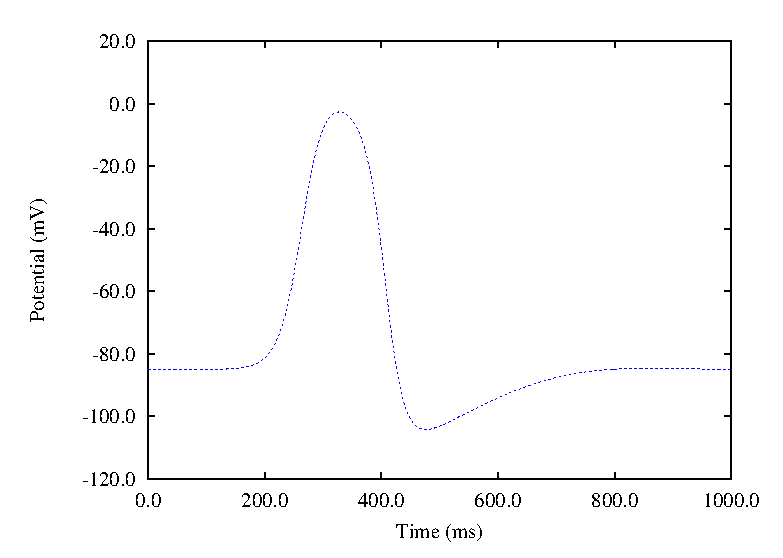
\includegraphics[width=\textwidth]{cardiac_electrophysiology/epsfiles/FHNVm.eps}
    \caption{}
  \end{subfigure}
  \hfill
  \begin{subfigure}[b]{0.45\linewidth}
    \centering
    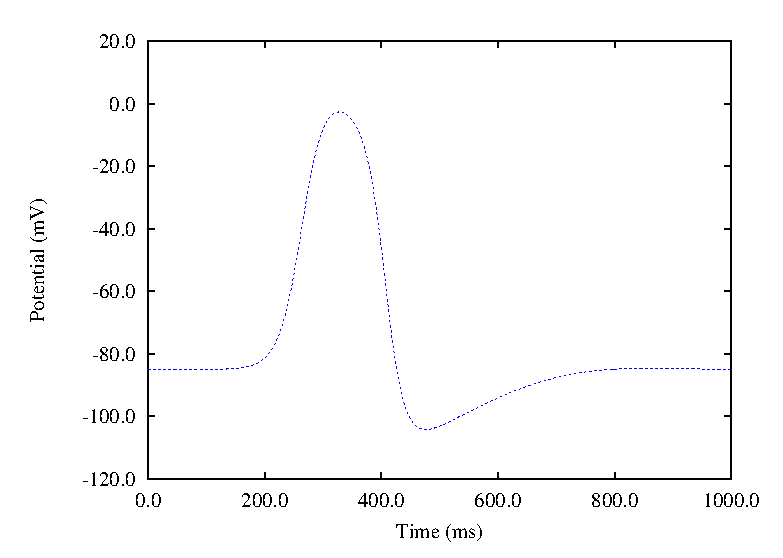
\includegraphics[width=\textwidth]{cardiac_electrophysiology/epsfiles/FHNVm.eps}
    \caption{}
  \end{subfigure}
  \caption[Traces from a single cell using the FitzHugh-Nagumo ionic current
  model]{Traces from a single cell using the FitzHugh-Nagumo ionic current
    model. Figure(a) shows the generated action potential and Figure(b) shows
    the recovery variable.}
  \label{fig:FHN_1_cell_traces}
\end{figure}
%
%===================================================================
\subsection{The modified FitzHugh-Nagumo model}
\label{The_modified_FitzHugh-Nagumo_Model}
%===================================================================
In the same paper as the original model was described \citeasnoun{rogers:1994a} described
some modifications to the model designed to generate a more realistic action
potential increasing the velocity of the upstroke and removing the large
hyperpolarization at the end of the action potential. The equation for the
ionic current was changed by multiplying the $c_2$ term by the normalised
potential. 
\begin{equation}
  I_{ion} = c_1 u \pbrac{u - \alpha} \pbrac{u - 1} + c_2 u \nu
  \label{eqn:mod_FHN_excitation_equation}
\end{equation}
The parameters which were used in the model were also updated. Alterations are
shown in \tabref{tab:mod_FitzHugh-Nagumo_Model_Params}.
\begin{table}[hbtp] \centering
  \begin{tabular}{|c|c|c|}
    \hline
    \emph{Parameter} & \emph{Units} & \emph{Value} \\ 
    \hline
    \hline 
    $c_1$ & $\uA\unitseparator\mm^{-2}$ & $0.26$ \\
    $c_2$ & $\uA\unitseparator\mm^{-2}$ & $0.1$ \\
    $b$ & $\pms$ & $0.013$ \\
    $d$ & $dimensionless$ & $0.8$ \\
    \hline
  \end{tabular}
  \caption[Adjusted parameters for the modified FitzHugh-Nagumo ionic current
  model]{Adjusted parameters for the modified FitzHugh-Nagumo ionic current model}
  \label{tab:mod_FitzHugh-Nagumo_Model_Params}
\end{table}
The resulting action potential and recovery variable traces are shown in
\figref{fig:FHNR_1_cell_traces}.
\begin{figure}[hbtp] 
  \centering
  \begin{subfigure}[b]{0.45\linewidth}
    \centering
    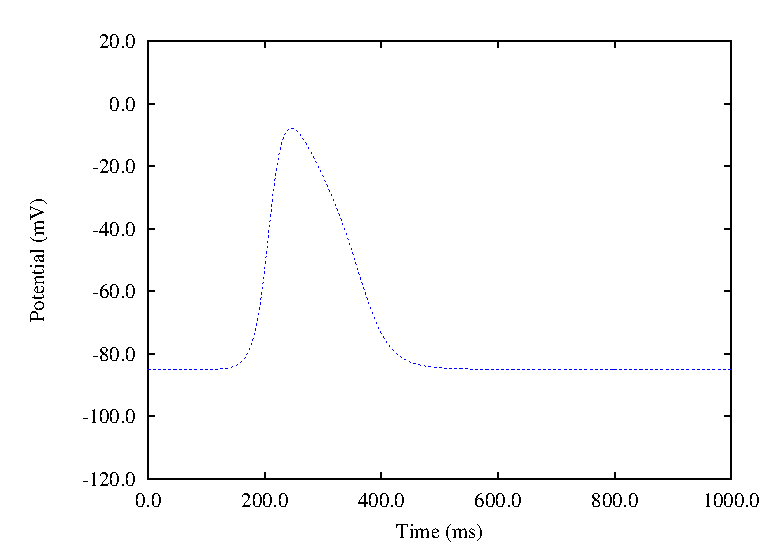
\includegraphics[width=\textwidth]{cardiac_electrophysiology/epsfiles/FHNRVm.eps}
    \caption{}
  \end{subfigure}
  \hfill
  \begin{subfigure}[b]{0.45\linewidth}
    \centering
    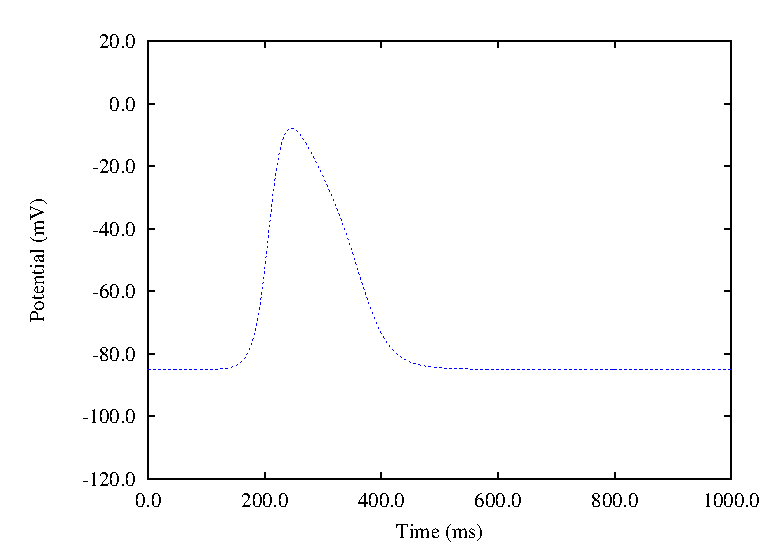
\includegraphics[width=\textwidth]{cardiac_electrophysiology/epsfiles/FHNRVm.eps}
    \caption{}
  \end{subfigure}
  \caption[Traces from a single cell using the modified FitzHugh-Nagumo ionic current
    model]{Traces from a single cell using the modified FitzHugh-Nagumo ionic current
    model. Figure(a) shows the generated action potential and Figure(b) shows
    the recovery variable.}
  \label{fig:FHNR_1_cell_traces}
\end{figure}
%
%===================================================================
\subsection{The van Capelle-Durrer model}
\label{The_van_Capelle-Durrer_Model}
%===================================================================
The van Capelle-Durrer model \cite{vancapelle:1980} follows the same general form as the
FitzHugh-Nagumo model with a single activation variable and a single recovery
variable but has the ability to add more complexity to the representation of
the parameters. The ionic current from the van Capelle-Durrer model is defined
to be
\begin{equation}
  I_{ion}=-Y \fnof{i_1}{V_m} - \pbrac{1-Y}\fnof{i_0}{V_m}
\end{equation}
where $\fnof{i_0}{V_m}$ and $\fnof{i_1}{V_m}$ are defined to be voltage
dependent currents and $Y$ is 
a dimensionless excitability parameter defined to be 
\begin{equation}
  \dby{Y}{t}=\dfrac{1}{T}\pbrac{\fnof{Y_{\infty}}{V_m}-Y}
\end{equation}
The $T$ parameter is a dimensionless time constant which may be used to easily scale the
duration of the action potential and $\fnof{Y_{\infty}}{V_m}$ is a voltage dependent
dimensionless variable which is the final value of the $Y$ parameter. In this
implementation of the model the $\fnof{Y_{\infty}}{V_m}$ was defined to be a piecewise
function. 
\begin{gather}
  \label{eqn:three_cases_of_Y_VCD}
  \begin{aligned}
  \fnof{Y_{\infty}}{V_m} &=
  \begin{cases}
    0 & \text{if $V_m < -80\mV$} \\
    1 & \text{if $V_m > -60\mV$} \\
    \pbrac{V_m+80}/20 & \text{otherwise}
  \end{cases}
  \end{aligned}
\end{gather}
A piecewise function was also chosen to represent $\fnof{i_1}{V_m}$.
\begin{gather}
  \label{eqn:three_cases_of_i1_VCD}
  \begin{aligned}
  \fnof{i_1}{V_m} &=
  \begin{cases}
    0.05+0.005\pbrac{V_m+70} 
      & \text{if $V_m < -70\mV$} \\
    0.06+0.00425V_m 
      & \text{if $V_m > 0\mV$} \\
    0.05+0.01\pbrac{V_m+70}/70 
      & \text{otherwise}
  \end{cases}
  \end{aligned}
\end{gather}
The $\fnof{i_0}{V_m}$ was not represented directly, instead it was defined to
be $\fnof{i_0}{V_m}=\fnof{i_1}{V_m}+\fnof{f}{V_m}$ where $\fnof{f}{V_m}$ was
defined by a piecewise function.
\begin{gather}
  \label{eqn: three_cases_of_f_VCD}
  \begin{aligned}
  \fnof{f}{V_m}=
  \begin{cases}
    0.0784+0.02\pbrac{V_m+74.3} 
      & \text{if $V_m < -74.3\mV$} \\
    -0.9884+0.0171\pbrac{V_m+27.8} 
      & \text{if $V_m > -27.8\mV$} \\
    a_fV_m^3+b_fV_m^2+c_fV_m+d_f 
      & \text{otherwise}
  \end{cases}
  \end{aligned}
\end{gather}
where
\begin{align*}
  a_f=& 3.837854\times 10^{-5}\\
  b_f=& 5.84649\times 10^{-3}\\
  c_f=& 0.2531834\\
  d_f=& 2.356256
\end{align*}
In this model $\fnof{i_0}{V_m}$, $\fnof{i_1}{V_m}$ and $\fnof{f}{V_m}$ have
units of $\uA\unitseparator\mm^{-2}$. The parameters used in the model are
given in \tabref{tab:VCD_Model_Params}.
\begin{table}[hbtp] \centering
  \begin{tabular}{|c|c|c|}
    \hline
    \emph{Parameter} & \emph{Units} & \emph{Value} \\ 
    \hline
    \hline 
    $V_m\pbrac{initial}$ & $\mV$ & $-78.6$ \\
    $Y\pbrac{initial}$ & $dimensionless$ & $0.07$ \\
    $T$ & $\ms$ & $50$ \\
    $C_m$ & $\uF\unitseparator\mm^{-2}$ & $0.01$ \\
    $A_m$ & $\mm^{-1}$ & $200$ \\
    \hline
  \end{tabular}
  \caption[Typical parameters for the van Capelle-Durrer ionic current model]{Typical
    parameters for the van Capelle-Durrer ionic current model}
  \label{tab:VCD_Model_Params}
\end{table}

Traces of both the action potential and the recovery variable $Y$ are shown in
\figref{fig:VCD_1_cell_traces}.  
\begin{figure}[hbtp] 
  \centering
  \begin{subfigure}[b]{0.45\linewidth}
    \centering
    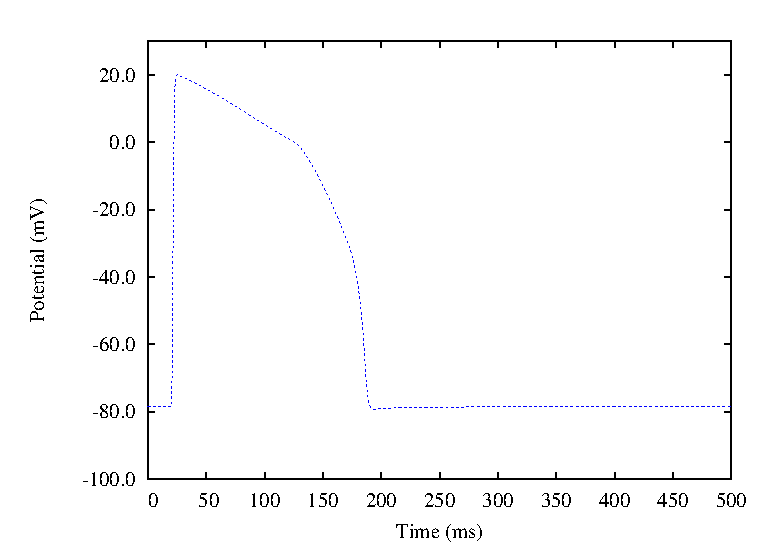
\includegraphics[width=\textwidth]{cardiac_electrophysiology/epsfiles/VCDVm.eps}
    \caption{}
  \end{subfigure}
  \hfill
  \begin{subfigure}[b]{0.45\linewidth}
    \centering
    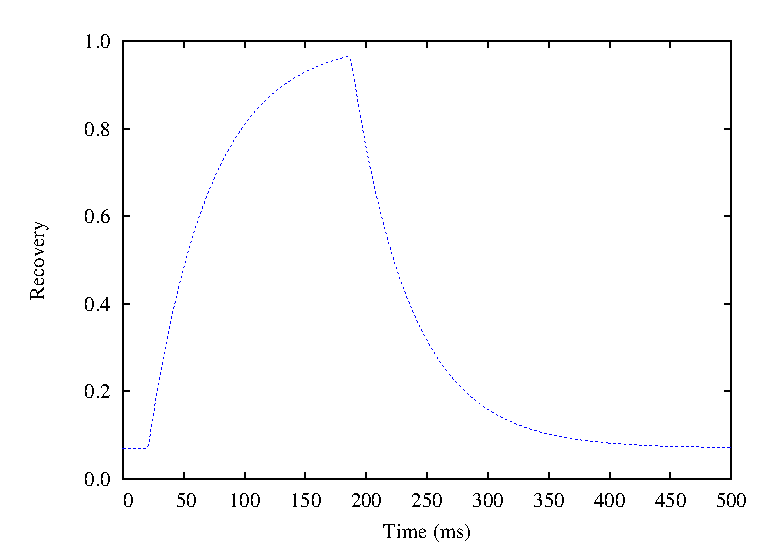
\includegraphics[width=\textwidth]{cardiac_electrophysiology/epsfiles/VCDRecov.eps}
    \caption{}
  \end{subfigure}
  \caption[Traces from a single cell using the van Capelle-Durrer ionic current
  model]{Traces from a single cell using the van Capelle-Durrer ionic current
    model. Figure(a) shows the generated action potential and Figure(b) shows
    the recovery variable.}
  \label{fig:VCD_1_cell_traces}
\end{figure}




\section{The Bidomain Model}
\label{sec:bidomain-model}

The complete model of cardiac activation would be one in which an
accurate model is formulated for each type of muscle cell.  The model
would completely describe the structure of the cell and detail every
aspect of its electrophysiological function down to a molecular level,
as well as the mechanical and energetic processes involved if this
information was required.  This cellular model would then be inserted
into an anatomically accurate description of the global cardiac
geometry, and solved on a cell-by-cell basis over the cardiac volume.
There are many reasons why such a model has not yet been constructed.
Firstly, it is difficult to obtain an accurate model of cell function.
Many of the membrane processes are still being quantified, if they are
known at all.  Secondly, an anatomically accurate definition of the
cardiac geometry is still incomplete.  Difficulties exist in measuring
the position of the ventricular endocardium, and many models only
describe the ventricular myocardium but not the atrial tissue or
accessory structures.  Coupled with this is a lack of a complete
description of the cellular structure.  The Auckland model is the most
detailed and accurate ventricular microstructural model to date, yet
it has little information on the Purkinje network, and none at all on
the atrial tissues.  The process of propagation is again only
partially understood, and a model describing even the conductivities
in the orthogonal microstructural directions is yet to be formulated.
Similar models of the energetic function and the passive and active
mechanics are still under construction, and the concept of being able
to couple the various components together in a total model is only
beginning to be looked at.  Even given the availability of this vast
amount of information, there would still be one requirement lacking.
Existing computational resources are barely adequate to solve a small
region of tissue.  \citeasnoun{spach:pilkington:1993} have developed a
model solving activation equations for individual cells for a
two-dimensional sheet model containing between 25,000 and 85,000
cells.  Even though there is only a small number of cells in a 2D
preparation, and the ionic model used is not the most complex
presently available, the model requires the use of a high-performance
supercomputer in order to solve the problem.  While computational
speeds are doubling approximately every eighteen months, a complete
model involving all cardiac processes is still a long way from being
computationally tractable.  Given that the current state of knowledge
and the current computational capabilities preclude the use of a model
completely representing the current state of knowledge of cardiac
activation, we need to determine what level of detail is feasible yet
sufficiently realistic so as to allow the investigation of various
abnormal phenomena.  The empirical models are no longer appropriate as
they ignore the cellular processes.  One commonly used method is to
use a macroscopic model which uses a volume-averaged approach, known
as the \emph{bidomain model}.  This model averages the electrical
properties over some length scale which is greater than that of a
single cell.  In doing this with an appropriate choice of length
scale, the effect of cell junctions on propagation can be ignored, and
the discrete cellular structure may be replaced with a uniformly
continuous structure.  There are problems with this approach.  If
discrete cellular effects play a significant role in the propagation
of activation, then either this will need to be incorporated or a new
model will need to be constructed.  Alternatively, if a macroscopic
model can provide results which are a reasonable approximation to the
explicit microscopic model then the averaged model may be justified.

\subsection{Definition of the Bidomain Framework}

The physical arrangement of cardiac cells has led to the belief that the heart
has electrical properties that are the same as a syncytium.  Experimental work
by \citeasnoun{weidmann:1970} and \citeasnoun{clerc:1976} on mammalian cardiac
tissue confirmed that propagation either along the fibre axis or transverse to
it produced results like a one-dimensional cable.  Cable theory defines
propagation along a membrane between two distinct spaces.  By extending
standard one-dimensional cable theory to two or three dimensions gives rise to
the bidomain model.

The concepts behind the bidomain model were first proposed by
\citeasnoun{schmitt:1969} who suggested that two interpenetrating domains could
be used to describe cardiac tissue, one representing volume-averaged
quantities in the intracellular space and one for those of the extracellular
space.  A mathematical formulation of this proposal was constructed in several
theses and papers by \citeasnoun{tung:1978}, \citeasnoun{plonsey:1984},
\citeasnoun{miller:1978a} and others.  The bidomain model has been adopted by
many other researchers in one form or another due to its convenience and
simplicity.  The model is discussed more fully in review papers by
\citeasnoun{henriquez:1993} and \citeasnoun{plonsey:1987}.  

Different papers give different names to the various regions that are part of
the bidomain model.  The names that we have chosen reflect the generally
accepted definitions (as given by \citeasnoun{krassowska:1994}) which tie in
with those that physiologists would use to describe cellular structure.  When
developing an activation model which is designed to be coupled with other
models, it is necessary to maintain consistent definitions and distinctly
identify each region.

The bidomain framework defines two domains which make up the cellular matrix.
The \emph{intracellular domain}, given the subscript ``$i$'', is the region
inside the cells, and the \emph{extracellular domain} with subscript ``$e$''
is the region between cells.  These two domains are interpenetrating which
means that they coexist at all points in space.  Therefore the properties and
state of the tissue at each point have separate components related to each
domain with appropriate subscripts.  For example, a single point in space will
have a tensor quantity associated with it defining the conductivity in each of
the intracellular and extracellular spaces.  The intracellular and
extracellular domains are separated by the cell membrane at all points, and
all current flow between the two domains occurs solely through the cell
membrane.  Because of the continuum approach to the physiology of the tissue,
this transmembrane current is volume-averaged.  This averaging approach is
required so that a length scale can be chosen such that the averaging produces
little loss of information.  Additionally, a third domain may be defined
consisting of all regions outside of the cardiac muscle, such as the bath that
the tissue is in, or the tissues within the torso cavity.  This domain is
referred to as the \emph{extramyocardial (outside) region} and given the
subscript ``$o$''.  \possessivecite{krassowska:1994} paper simply refers to
this region as ``outside'', but in a coupled problem it is unsure whether this
should refer to a region outside the heart or outside the body.  This naming
convention is illustrated in \figref{fig:bidomain-diagram}.
\begin{figure}[tb]
  \begin{center}
    \leavevmode
    \input{electrocardiology/figs/bidomain-diagram.pstex}
    \caption[The bidomain model]{The bidomain model.}
    \label{fig:bidomain-diagram}
  \end{center}
\end{figure}

Some authors (including \citeasnoun{pollard:pilkington:1993},
\citeasnoun{henriquez:1993}, \citeasnoun{plonsey:1987} and others), define the
regions differently.  In particular, what we term the extramyocardial region
is defined as the extracellular space, and what we call the extracellular
domain is called the \emph{interstitial domain}, often with ``extracellular''
also written in parentheses afterwards.  This causes some confusion in the
definitions of what constitutes extracellular space, and is inconsistent with
the standard physiological definition of the extracellular matrix being the
connective support structure and myoplasm surrounding cells.  Therefore it
seems best not to use the term ``interstitial'' at all, but to reserve the
word ``extracellular'' for use in describing structure that is part of the
extracellular matrix, and use another term for the medium surrounding the
tissue, which in this case we have chosen to call ``extramyocardial''.  This
agrees also with the tissue definitions of \citeasnoun{clerc:1976} in his
study of tissue conductivities which is cited as a definition for these terms
by \citeasnoun{pollard:pilkington:1993}.  It is true that the extramyocardial
space is also technically extracellular, but it is not (by definition) part of
the cardiac tissue structure, and because it is often not used in many
bidomain simulations, it is sensible to use another name for this region.
Some authors\cite{plonsey:1987} also use the subscript ``$o$'' for the
extracellular space, but this seems much less standard, and is similarly
confusing.

The bidomain model describes current flow through the cell membrane in a
space-averaged sense.  Instead of modelling a discrete cellular structure, the
bidomain constructs a continuum model with effective conductivity tensors
which is governed by continuous partial differential equations.  

\subsection{Mathematical Derivation of the Bidomain Model}

The most substantial mathematical description of the bidomain model is found
in the review paper by \citeasnoun{henriquez:1993}, which presents a formal
definition of the model from its origins in the core conductor model, and
outlines many of the approximations that can be made under certain
assumptions.

The bidomain equations may be derived in several ways depending on what
variables are wanted to solve for. This derivation yields equations for the
extracellular potential and the transmembrane potential while it is also
possible to generate equations for the intracellular and extracellular
potentials. The key definition in the bidomain equations is the definition of the
potential difference across the cell membrane which is known as the
transmembrane potential and given the symbol $V_m$.
\begin{equation}
  V_m = \phi_i - \phi_e
  \label{eqn:Vm_init_definition}
\end{equation}
Here $\phi_i$ is the potential in the intracellular domain and $\phi_e$ is the
potential in the extracellular domain. A schematic diagram of a bidomain
system is shown in \figref{fig:bidomain-diagram}. Ohm's law was  used
to calculate the intracellular and extracellular current densities. It is
assumed that the only current flow between the 
extracellular and extramyocardial space occurs through the boundary conditions
imposed on the domains.
\begin{align}
  V=&JR \nonumber \\
  J=&\dfrac{1}{R} V 
  \label{eqn:Ohms_Law}
\end{align}
Here $V$ is a voltage, $J$ is a current and $R$ is a resistance. Voltages
result from potential gradients so $V=\grad{\phi}$ may be substituted. In
addition to this the $\dfrac{1}{R}$ term may be written as a conductivity,
$\sigma$ which has units of $\mS$. \Eqnref{eqn:Ohms_Law} is then written for
the two domains as 
\begin{align}
  J_i=& - \sigma_i \grad{\phi_i} 
  \label{eqn:J_i_from_Ohms_Law} \\
  J_e=& - \sigma_e \grad{\phi_e}
  \label{eqn:J_e_from_Ohms_Law}
\end{align}
The negative signs in \eqnref{eqn:J_i_from_Ohms_Law} and
\eqnref{eqn:J_e_from_Ohms_Law} are necessary to ensure that current flows are
in the correct direction from regions of high potential to areas of low
potential. Any current which leaves one domain must cross the cell membrane and flow
into the other domain. This means that the change in current density in each
of the domains must be equal in magnitude but opposite in sign. The change in
current density in each domain is also equal to the current density across the
membrane.
\begin{equation}
  - \dotprod{\grad}{J_i} = \dotprod{\grad}{J_e} = A_mI_m
  \label{eqn:equal_current_densities}
\end{equation}
Here $A_m$ is defined to be the surface to volume ratio of the cell membrane
with units of $\pmm$ and
$I_m$ is the transmembrane current density per unit area which has units of
$\mS\unitseparator\mm^{-2}$. Combining
\eqnref{eqn:J_i_from_Ohms_Law}, \eqnref{eqn:J_e_from_Ohms_Law} and
\eqnref{eqn:equal_current_densities}, two equations were generated which
represent the conservation of current densities.
\begin{align}
  \dotprod{\grad}{\pbrac{\sigma_i \grad{\phi_i}}} =& A_mI_m
  \label{eqn:current_dens_conserv_1} \\
  \dotprod{\grad}{\pbrac{\sigma_e \grad{\phi_e}}} =& -A_mI_m
  \label{eqn:current_dens_conserv_2}
\end{align}
This implies that
\begin{equation}
  \dotprod{\grad}{\pbrac{\sigma_i \grad{\phi_i}}} = 
  -\dotprod{\grad}{\pbrac{\sigma_e \grad{\phi_e}}}
  \label{eqn:current_dens_conserv_3}
\end{equation}
Subtracting $\dotprod{\grad}{\pbrac{\sigma_i \grad{\phi_e}}}$ from both sides yields
\begin{equation}
  \dotprod{\grad}{\pbrac{\sigma_i \grad{\phi_i}}} 
  -\dotprod{\grad}{\pbrac{\sigma_i \grad{\phi_e}}} =
  -\dotprod{\grad}{\pbrac{\sigma_e \grad{\phi_e}}} 
  -\dotprod{\grad}{\pbrac{\sigma_i \grad{\phi_e}}}
  \label{eqn:current_dens_conserv_4}
\end{equation}
Using \eqnref{eqn:Vm_init_definition}, \eqnref{eqn:current_dens_conserv_4} can
be rewritten as
\begin{equation}
  \dotprod{\grad}{\pbrac{\sigma_i \grad{V_m}}} = 
  -\dotprod{\grad}{\pbrac{\pbrac{\sigma_i + \sigma_e} \grad{\phi_e}}}
  \label{eqn:first_bidomain_equation}
\end{equation}
This equation is usually refered to as the one of the two bidomain
equations which is used to solve for the extracellular potential given a
transmembrane potential distribution. The current flow across the
membrane, $I_m$ may be described by a time dependent capacitive current and an
ionic current
\begin{equation}
  I_m = C_m \delby{V_m}{t} + I_{ion}
  \label{eqn:membrane_current_flow}
\end{equation}
where $C_m$ is a membrane capacitance per unit area and $I_{ion}$ is the sum
of all ionic currents. The models used to 
represent the ionic
current component are presented in
\secref{sec:biophysical_models_of_cardiac_cells} and
\secref{sec:Simplified_models_of_cardiac_cells}. Combining
\eqnref{eqn:current_dens_conserv_1} and \eqnref{eqn:membrane_current_flow}
gives the following equation.
\begin{equation}
  \dotprod{\grad}{\pbrac{\sigma_i \grad{\phi_i}}} =
   A_m \pbrac{C_m \delby{V_m}{t} + I_{ion}}
  \label{eqn:membrane_current_flow_conserv}
\end{equation}
To convert \eqnref{eqn:membrane_current_flow_conserv} to have $V_m$ as the
dependent variable, $\dotprod{\grad}{\pbrac{\sigma_i \grad{\phi_e}}}$ is
added and subtracted from the left hand side of the equation.
\begin{equation}
  \dotprod{\grad}{\pbrac{\sigma_i \grad{\phi_i}}} -
  \dotprod{\grad}{\pbrac{\sigma_i \grad{\phi_e}}} +
  \dotprod{\grad}{\pbrac{\sigma_i \grad{\phi_e}}} =
   A_m \pbrac{C_m \delby{V_m}{t} + I_{ion}}
  \label{eqn:membrane_current_flow_conserv2}
\end{equation}
Using \eqnref{eqn:Vm_init_definition}
\eqnref{eqn:membrane_current_flow_conserv2} may be expressed as 
\begin{equation}
  \dotprod{\grad}{\pbrac{\sigma_i \grad{V_m}}} +
  \dotprod{\grad}{\pbrac{\sigma_i \grad{\phi_e}}} =
   A_m \pbrac{C_m \delby{V_m}{t} + I_{ion}}
  \label{eqn:second_bidomain_equation}
\end{equation}
which is known as the second of the bidomain equations and is used to update
the transmembrane potential at each time. It is possible for an
external stimulus current to be applied to either domain which gives the two
bidomain equations as
\begin{align}
  \dotprod{\grad}{\pbrac{\pbrac{\sigma_i + \sigma_e} \grad{\phi_e}}} =&
  -\dotprod{\grad}{\pbrac{\sigma_i \grad{V_m}}} +I_{s1}\\
  \dotprod{\grad}{\pbrac{\sigma_i \grad{V_m}}} +
  \dotprod{\grad}{\pbrac{\sigma_i \grad{\phi_e}}} =&
   A_m \pbrac{C_m \delby{V_m}{t} + I_{ion}} -I_{s2}
  \label{eqn:starting_bidomain_equations}
\end{align}
The extracellular domain is sometimes assumed to be highly conducting or the
domains are assumed to be equally anisotropic in an
effort to reduce the bidomain equations to a single domain hence reducing the
amount of computational effort required to solve the problem. The reduced
equation is known as the monodomain equation and is written as
\begin{equation}
  \dotprod{\grad}{\pbrac{\sigma \grad{V_m}}} =
   A_m \pbrac{C_m \delby{V_m}{t} + I_{ion}} -I_{s}
  \label{eqn:starting_monodomain_equation}  
\end{equation}
where the transmembrane potential is equal to the intracellular potential as
the extracellular potential is effectively zero. The conductivity values in
both the monodomain and bidomain equations are represented at each point in
space by a tensor containing conductivities in the fibre, sheet and cross
sheet directions allowing spatially varying fully orthotropic conductivities
to be modelled. 
%
%===================================================================
\subsubsection{Boundary conditions}
%\label{sec:bidomain_Boundary_conditions}
%===================================================================
There has been some differences in the literature in the boundary conditions
which have been applied to the bidomain model \citeasnoun{krassowska:1994}. The boundary
conditions used here are the original boundary conditions specified
by \citeasnoun{tung:1978} and confirmed by \citeasnoun{krassowska:1994}. There is assumed to be no
current flow between the intracellular and extramyocardial domains so the
boundary condition applied to the boundaries on intracellular space may be
written as
\begin{equation}
  \dotprod{\sigma_i \grad \phi_i}{\vect{n}}=0
  \label{eqn:orig_int_bc}
\end{equation}
where $n$ is a unit outward normal vector. The $\phi_i$ parameter was not
explicitly represented in the formulation of 
the bidomain equations so the boudary condition was modified to become a
boundary condition on $V_m$ using \eqnref{eqn:Vm_init_definition}. Taking
gradients, multiplying through by $\sigma_i$ and then taking dot products with
a normal vector, 
\eqnref{eqn:Vm_init_definition} becomes
\begin{equation}
  \dotprod{\sigma_i \grad V_m}{\vect{n}} = \dotprod{\sigma_i \grad \phi_i}{\vect{n}} -
  \dotprod{\sigma_i \grad \phi_e}{\vect{n}} 
\end{equation}
where \eqnref{eqn:orig_int_bc} demonstrates the $\phi_i$ term to be zero so
the actual boundary condition on the transmembrane potential becomes
\begin{equation}
  \dotprod{\sigma_i \grad V_m}{\vect{n}} = -\dotprod{\sigma_i \grad \phi_e}{\vect{n}} 
  \label{eqn:actual_int_bc}
\end{equation}
The boundary conditions on the extracellular domain were set up as a current
balance between the domain and the surrounding extramyocardial regions. 
\begin{equation}
  \dotprod{\sigma_e \grad \phi_e}{\vect{n}}=-\dotprod{\sigma_o \grad \phi_o}{\vect{n}}
  \label{eqn:orig_ext_bc}
\end{equation}
The negative sign accounts for the direction of current flow where both sides
of the equation use the same unit normal vector. The boundary extracellular
potentials must also match the boundary extramyocardial potentials. 
\begin{equation}
  \phi_e = \phi_o
\end{equation}
If the tissue is not
surrounded by a medium combinations of flux and potential boundary conditions
may be used to represent the desired setup. For a bidomain simulation with
equal anisotropy ratios an analytic potential boundary condition \citeasnoun{henriquez:1993}
may be set which is equal to
\begin{equation}
  \phi_e=-\dfrac{\sigma_{if}\sigma_{ef}}{\sigma_{if}+\sigma_{ef}}
\end{equation}
where $\sigma_{if}$ is the intracellular conductivity in the fibre direction
and $\sigma_{ef}$ is the extracellular conductivity in the fibre direction.
The boundary condition which was applied to the monodomain equation stated
that there was no current flow out of the myocardial domain because no
connection exists between the intracellular domain and any surrounding medium.
\begin{equation}
  \dotprod{\sigma \grad V_m}{\vect{n}}=0
\end{equation}
%The reaction part of the bidomain equations was represented by $I_{ion}$ which
%is usually highly nonlinear. 

